\documentclass[aspectratio=169]{beamer}
\usepackage{lmodern}
%\usetheme{Madrid}
%\usecolortheme{giantoak}
\newcommand*\oldmacro{}
\let\oldmacro\insertshorttitle
\renewcommand*\insertshorttitle{\oldmacro\hfill\insertframenumber\,/\,\inserttotalframenumber}
\usepackage[framemethod=tikz]{mdframed}

%\usepackage{beamerthemesplit}
\usepackage{textpos}
\usepackage{pgf}
\usepackage{ulem}
%\logo{\pgfputat{\pgfxy(0,-.4)}{\pgfbox[right,base]{\includegraphics[height=1.0cm]{logo.jpg}}}}
%\newcommand{\nologo}{\setbeamertemplate{logo}{}}
\usepackage{booktabs}
\usepackage{graphicx}
\theoremstyle{principle}
\newtheorem*{principle}{Design Principle}


\titlegraphic{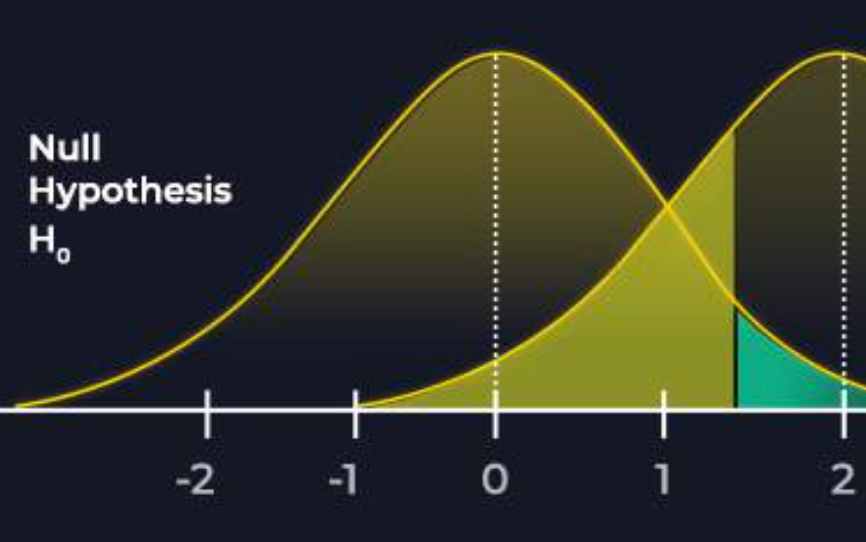
\includegraphics[width=1.0\paperwidth]{distros.png}}

\title{Amendments}
%\author[Jeremy Kedziora]{Wind Data Science Team\\
%\small{Uptake}}
\date{}

\begin{document}

%{
%%\nologo
%\begin{frame}
%    \maketitle
%\end{frame}
%}
%pages 1-7, 8-9, 14-15.


{
%  \usebackgroundtemplate{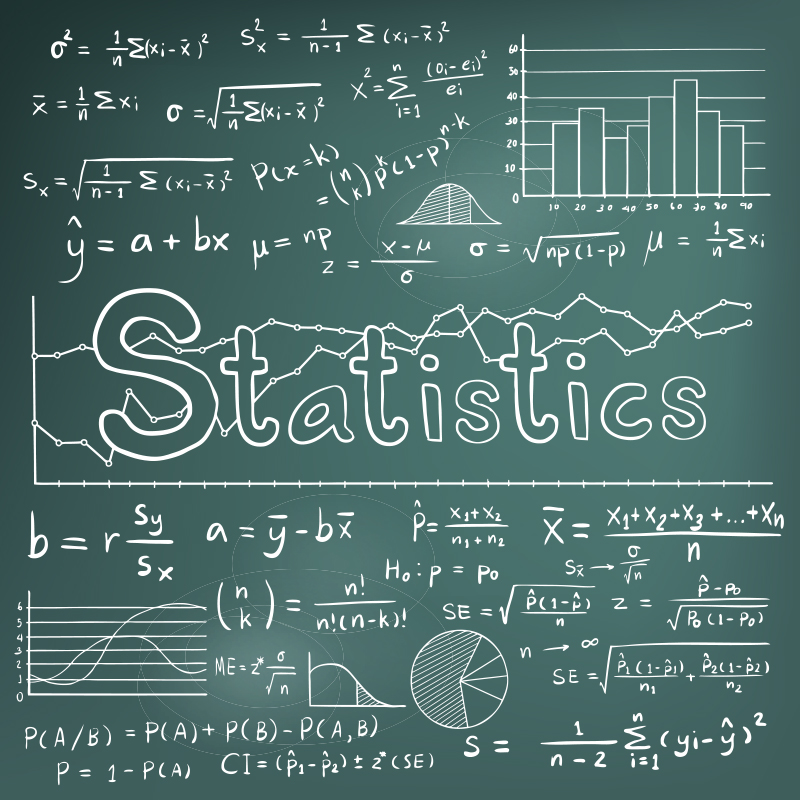
\includegraphics[width=1.0\paperwidth]{statistics-review.jpg}}
  \usebackgroundtemplate{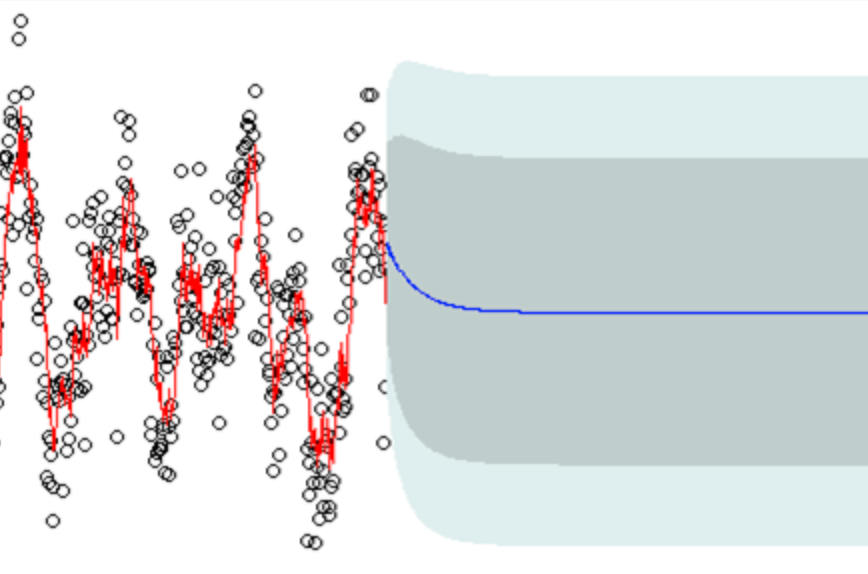
\includegraphics[scale=1.1]{oos.png}}
  \begin{frame}[plain]
  
\begin{mdframed}[tikzsetting={draw=white,fill=white,fill opacity=0.6,draw opacity=0.4,
               line width=0pt},backgroundcolor=none,leftmargin=20,
               rightmargin=20,innertopmargin=4pt]
\begin{center}
\Huge \textbf{Working Out of Sample}
\end{center}
\end{mdframed}

  \end{frame}
}

%most reliant on human cognition
%limited only by cognition
%hypothesis generating scheme often functioning as a gateway into more statistical analysis

%%@@@@@@@@@@@@@@@@@@@@@@@@@@@@@@@@@@@@@@@@@@@@@@@@@
%\begin{frame}
%\frametitle{Napoleon's Progress}
%\begin{center}
%
\includegraphics[scale=0.4]{experiment.png}
%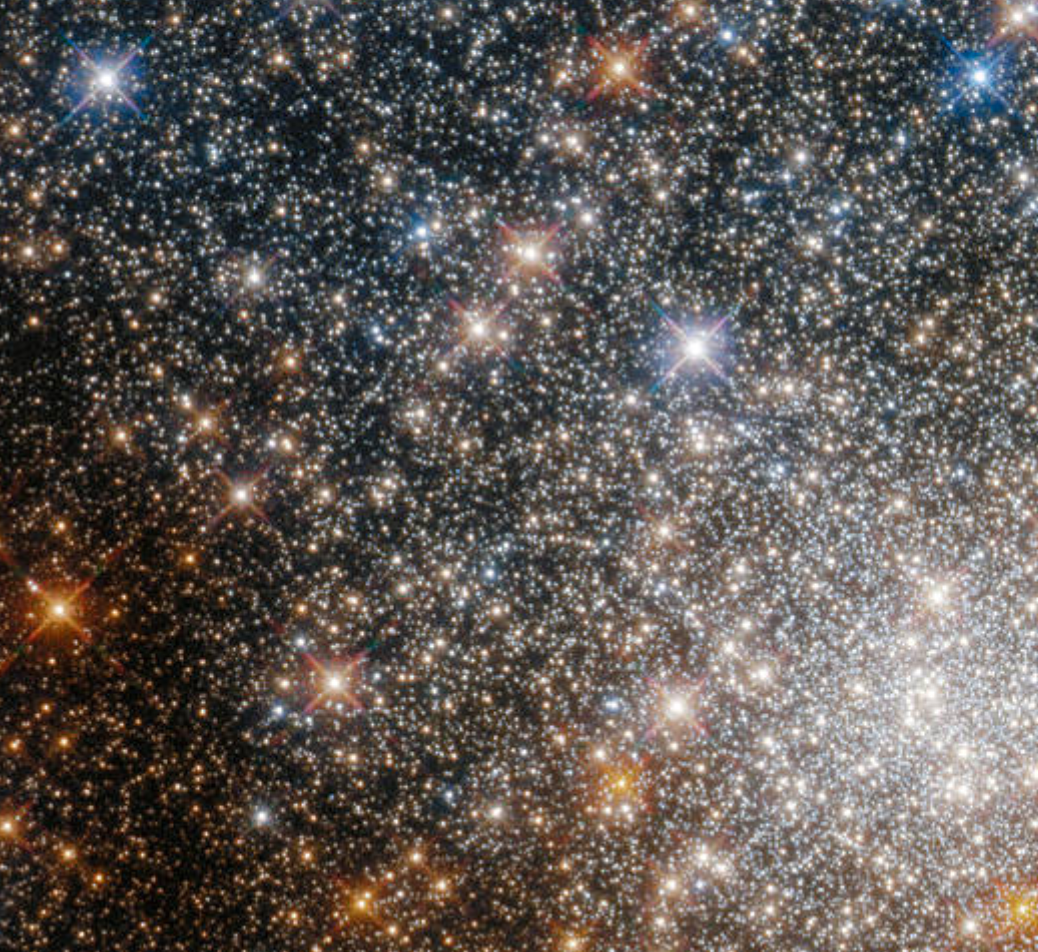
\includegraphics[scale=0.35]{stars.png}
%\end{center}
%
%\end{frame}

%@@@@@@@@@@@@@@@@@@@@@@@@@@@@@@@@@@@@@@@@@@@@@@@@@
\begin{frame}
\frametitle{Today:}

\begin{itemize}
\item Introduce the ideas of political forecasting;
\bigskip
\bigskip
\bigskip

\item Discuss these ideas in the context of the 2016 election;
\bigskip
\bigskip
\bigskip

\item Talk about out of sample work in relation model assessment.

\end{itemize}

\end{frame}

%@@@@@@@@@@@@@@@@@@@@@@@@@@@@@@@@@@@@@@@@@@@@@@@@@
\begin{frame}
\frametitle{Working out of sample}
\begin{itemize}
\item Major question: what does your model say about data not used to create it?
\bigskip
\bigskip
\bigskip

\item Two motivations for working out of sample:
\begin{enumerate}
\item \textbf{Forecasting} -- what does your model say about the future?
\begin{itemize}
\item Used to drawn conclusions and make inferences;
\item Model is not generally under evaluation;
\end{itemize}
\item \textbf{Assessment} -- does your model predict well outside of the data on which it was made?
\begin{itemize}
\item Used to evaluate the model and make sure it isn't `overfit' to the data it was made with;
\item Model is very much under evaluation!
\end{itemize}

\end{enumerate}

\end{itemize}

\end{frame}

%@@@@@@@@@@@@@@@@@@@@@@@@@@@@@@@@@@@@@@@@@@@@@@@@@
\begin{frame}

\begin{center}
\Huge\textbf{Forecasting -- what does your model say about the future?}\\
\end{center}

\end{frame}

%@@@@@@@@@@@@@@@@@@@@@@@@@@@@@@@@@@@@@@@@@@@@@@@@@
\begin{frame}
\frametitle{Let's forecast the 2016 Election -- whoops!}

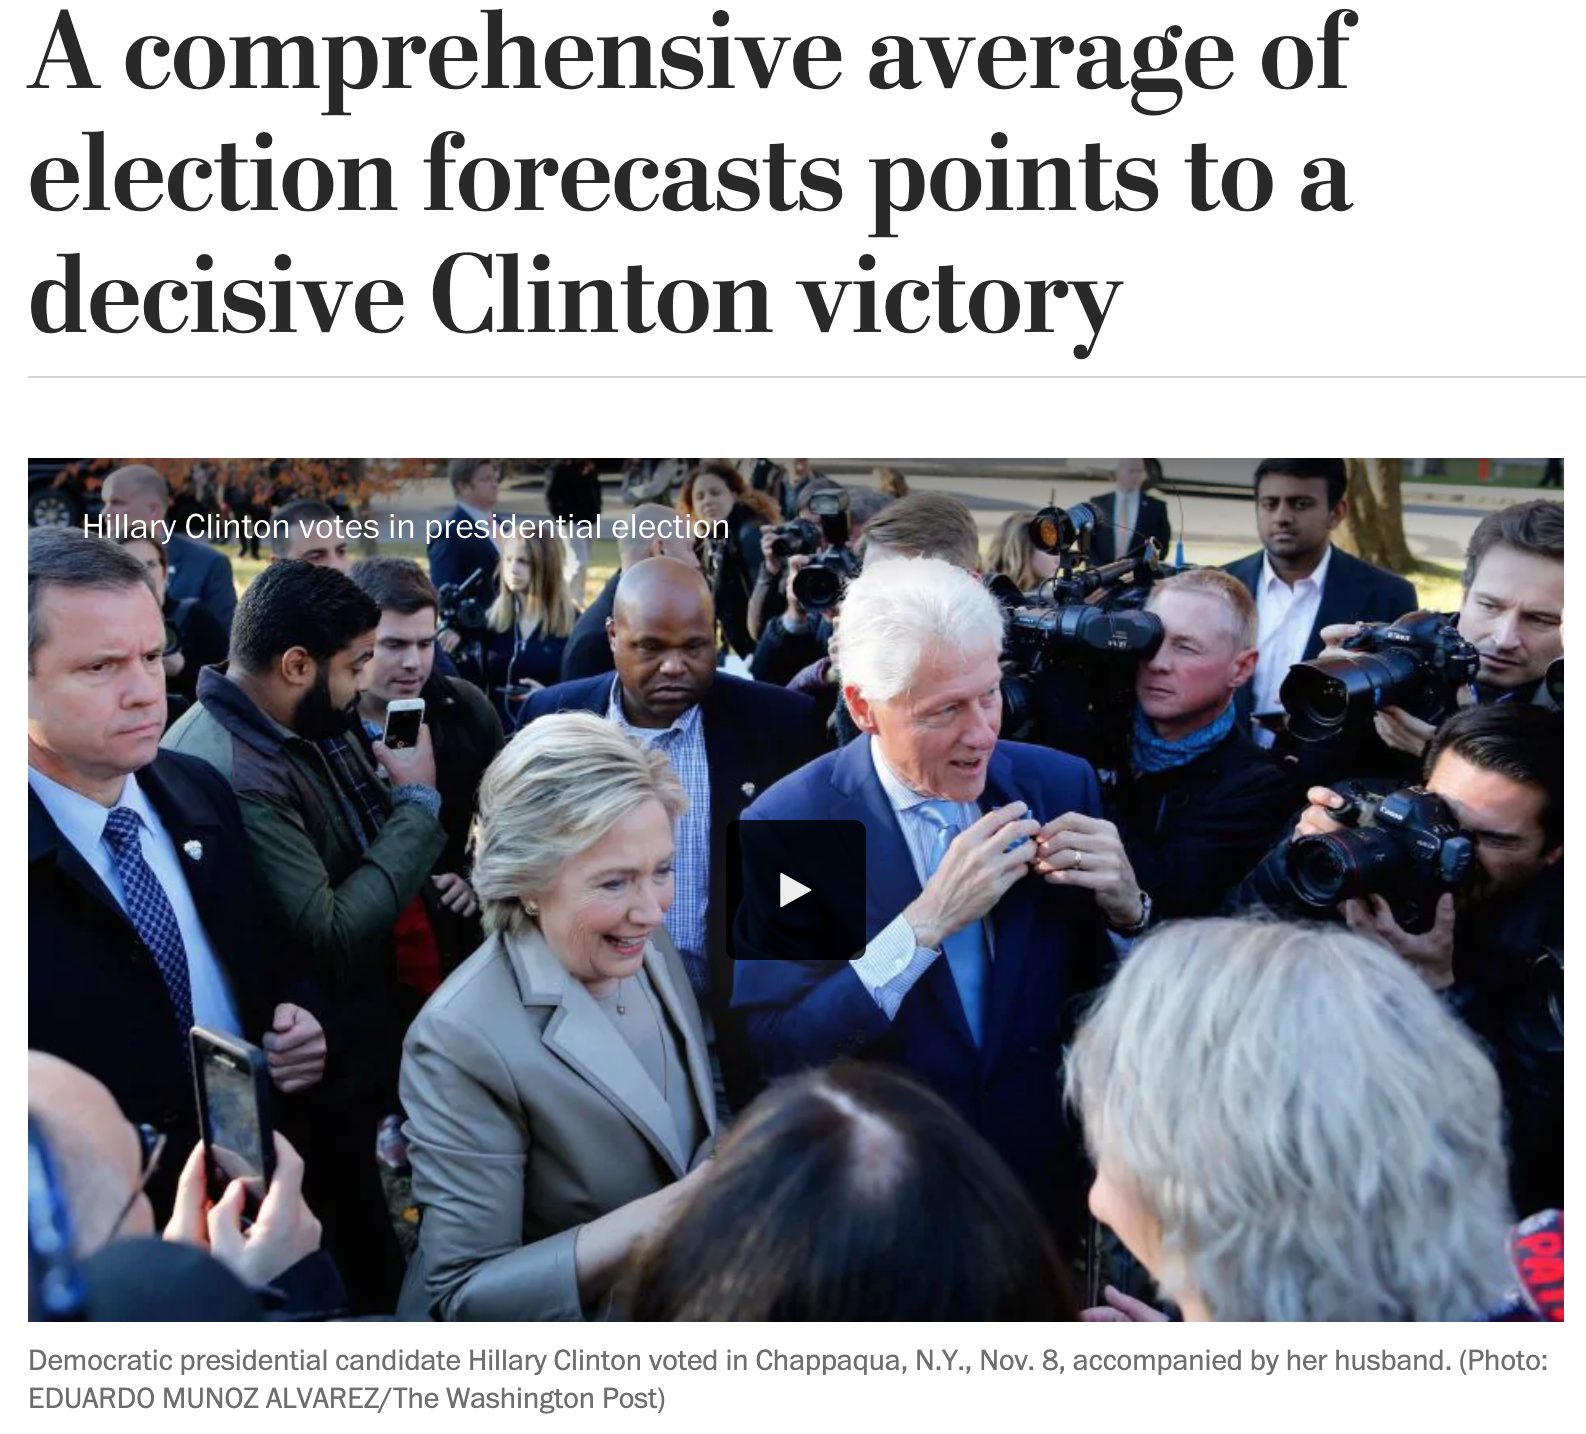
\includegraphics[scale=0.23]{oops-avg.png}
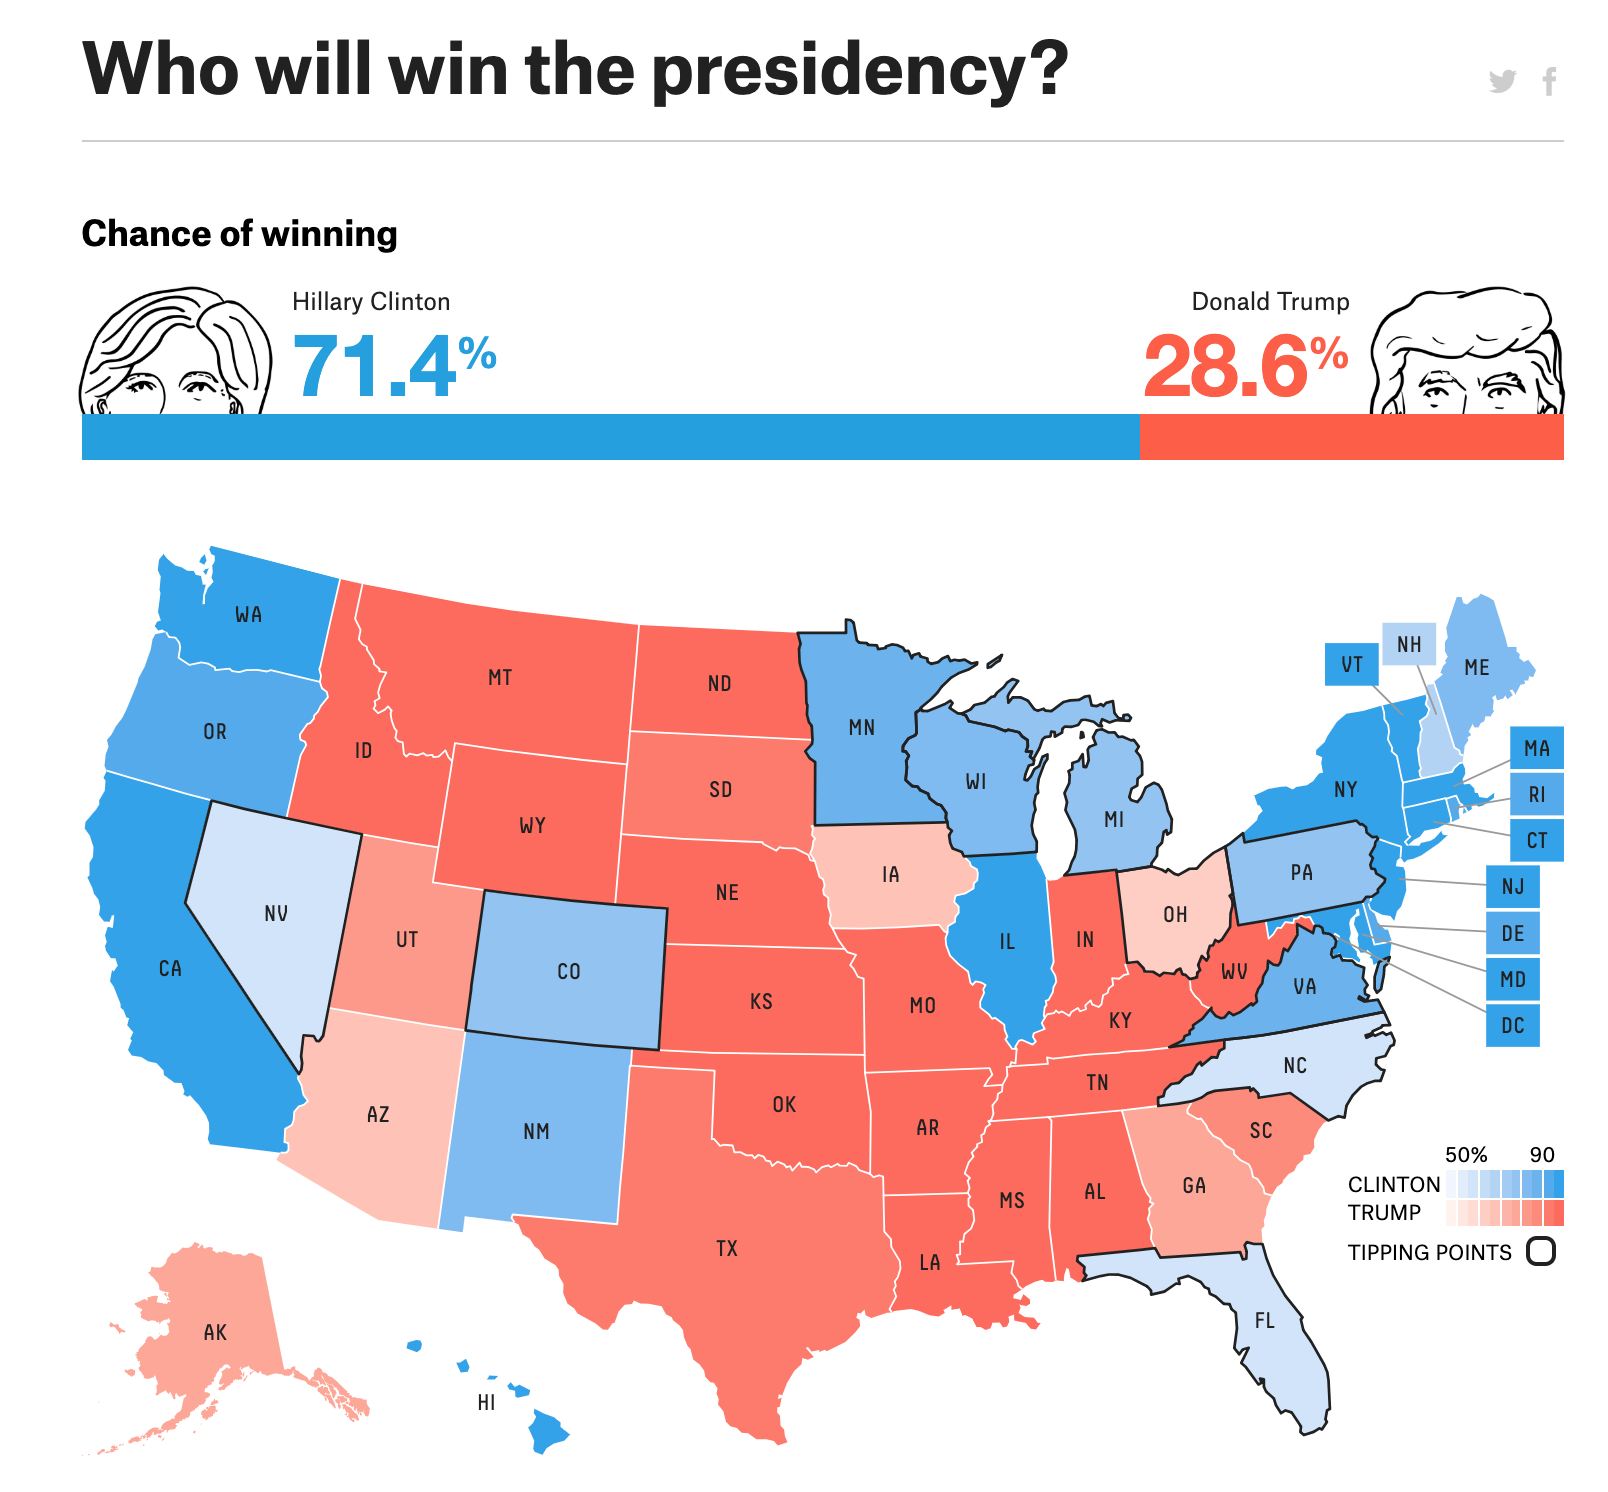
\includegraphics[scale=0.23]{oops-538.png}

\end{frame}

%@@@@@@@@@@@@@@@@@@@@@@@@@@@@@@@@@@@@@@@@@@@@@@@@@
\begin{frame}
\frametitle{FiveThirtyEight is a well known election forecasting model...}

\begin{itemize}
\item How does it work?  Some key facts that underpin how it uses data:
\begin{itemize}
\item Electoral college votes are allocated at state level;
\bigskip

\item National vote $\neq$ state vote $\Rightarrow$ national vote $\neq$ electoral college vote;
\bigskip

\item Popular vote $\neq$ electoral college vote;
\bigskip

\item Probability of winning $\neq$ Popular vote $\Rightarrow$ probability of winning $\neq$ vote percentage;
\bigskip
 
\item Shouldn't give a ``point prediction"—forecasts should incorporate \textbf{uncertainty}.
\end{itemize}
\end{itemize}

\end{frame}

%@@@@@@@@@@@@@@@@@@@@@@@@@@@@@@@@@@@@@@@@@@@@@@@@@
\begin{frame}

\begin{center}
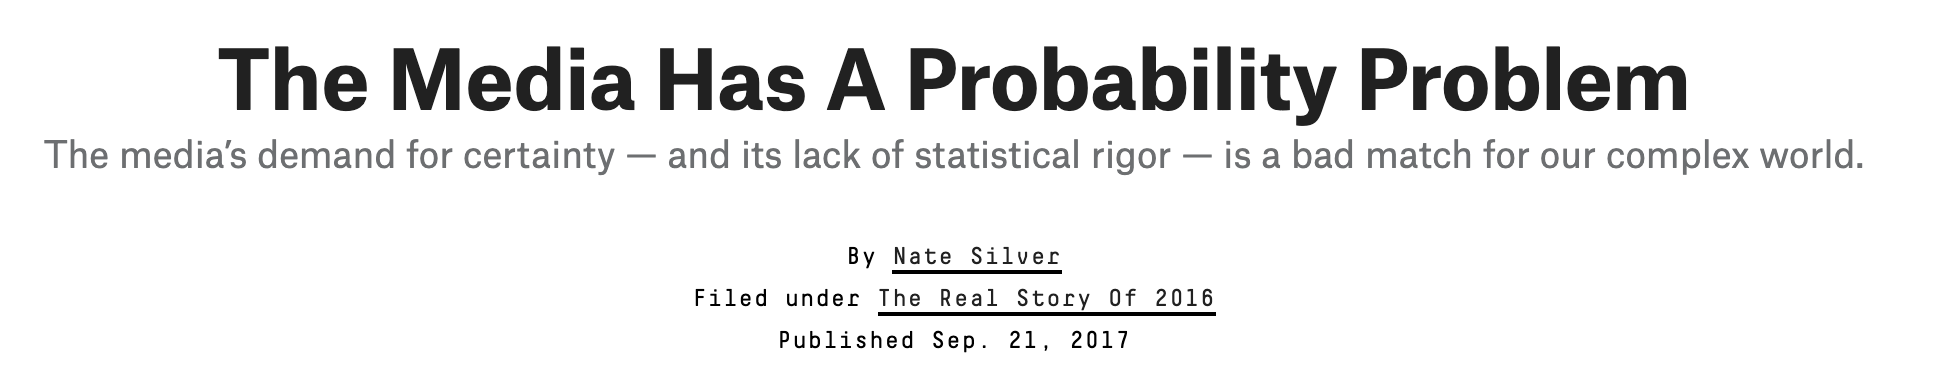
\includegraphics[scale=0.4]{prob-problem.png}
\end{center}

\end{frame}

%@@@@@@@@@@@@@@@@@@@@@@@@@@@@@@@@@@@@@@@@@@@@@@@@@
\begin{frame}

\begin{center}
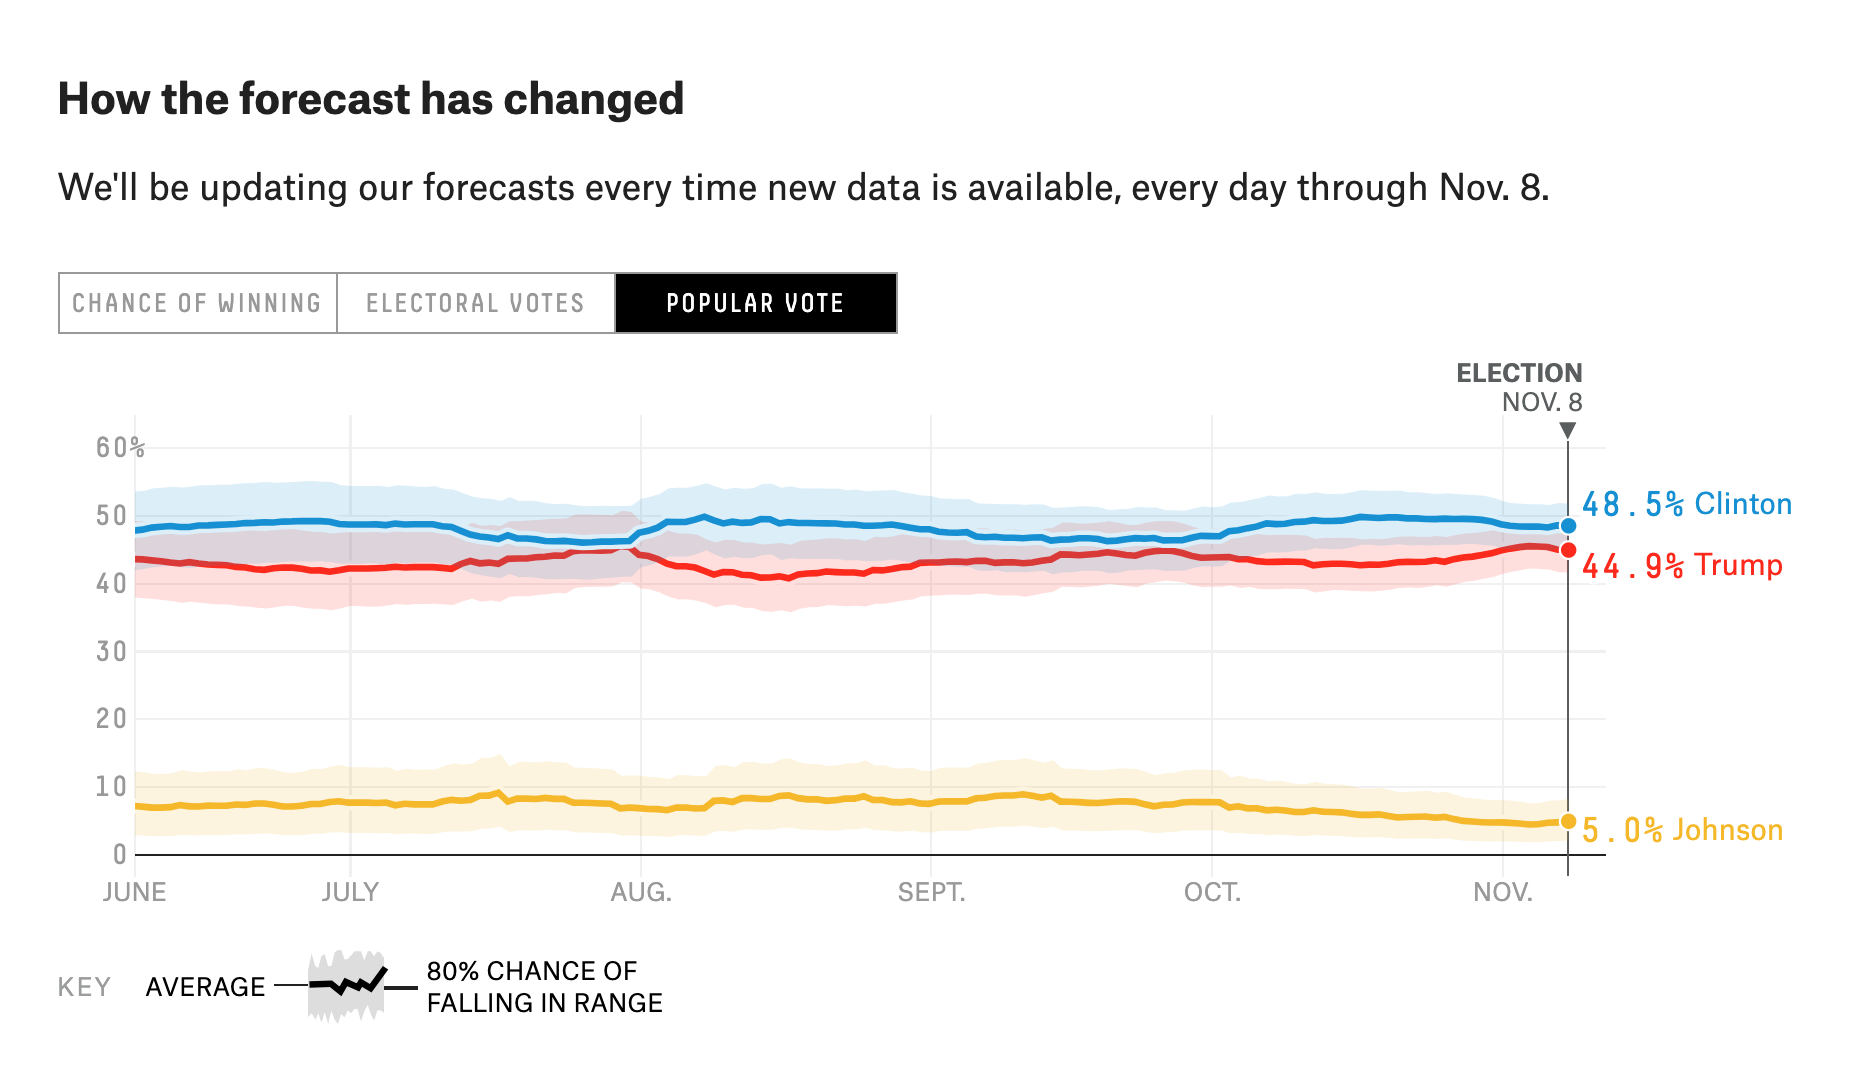
\includegraphics[scale=0.4]{forecast-pop.png}
\end{center}

\end{frame}

%@@@@@@@@@@@@@@@@@@@@@@@@@@@@@@@@@@@@@@@@@@@@@@@@@
\begin{frame}

\begin{center}
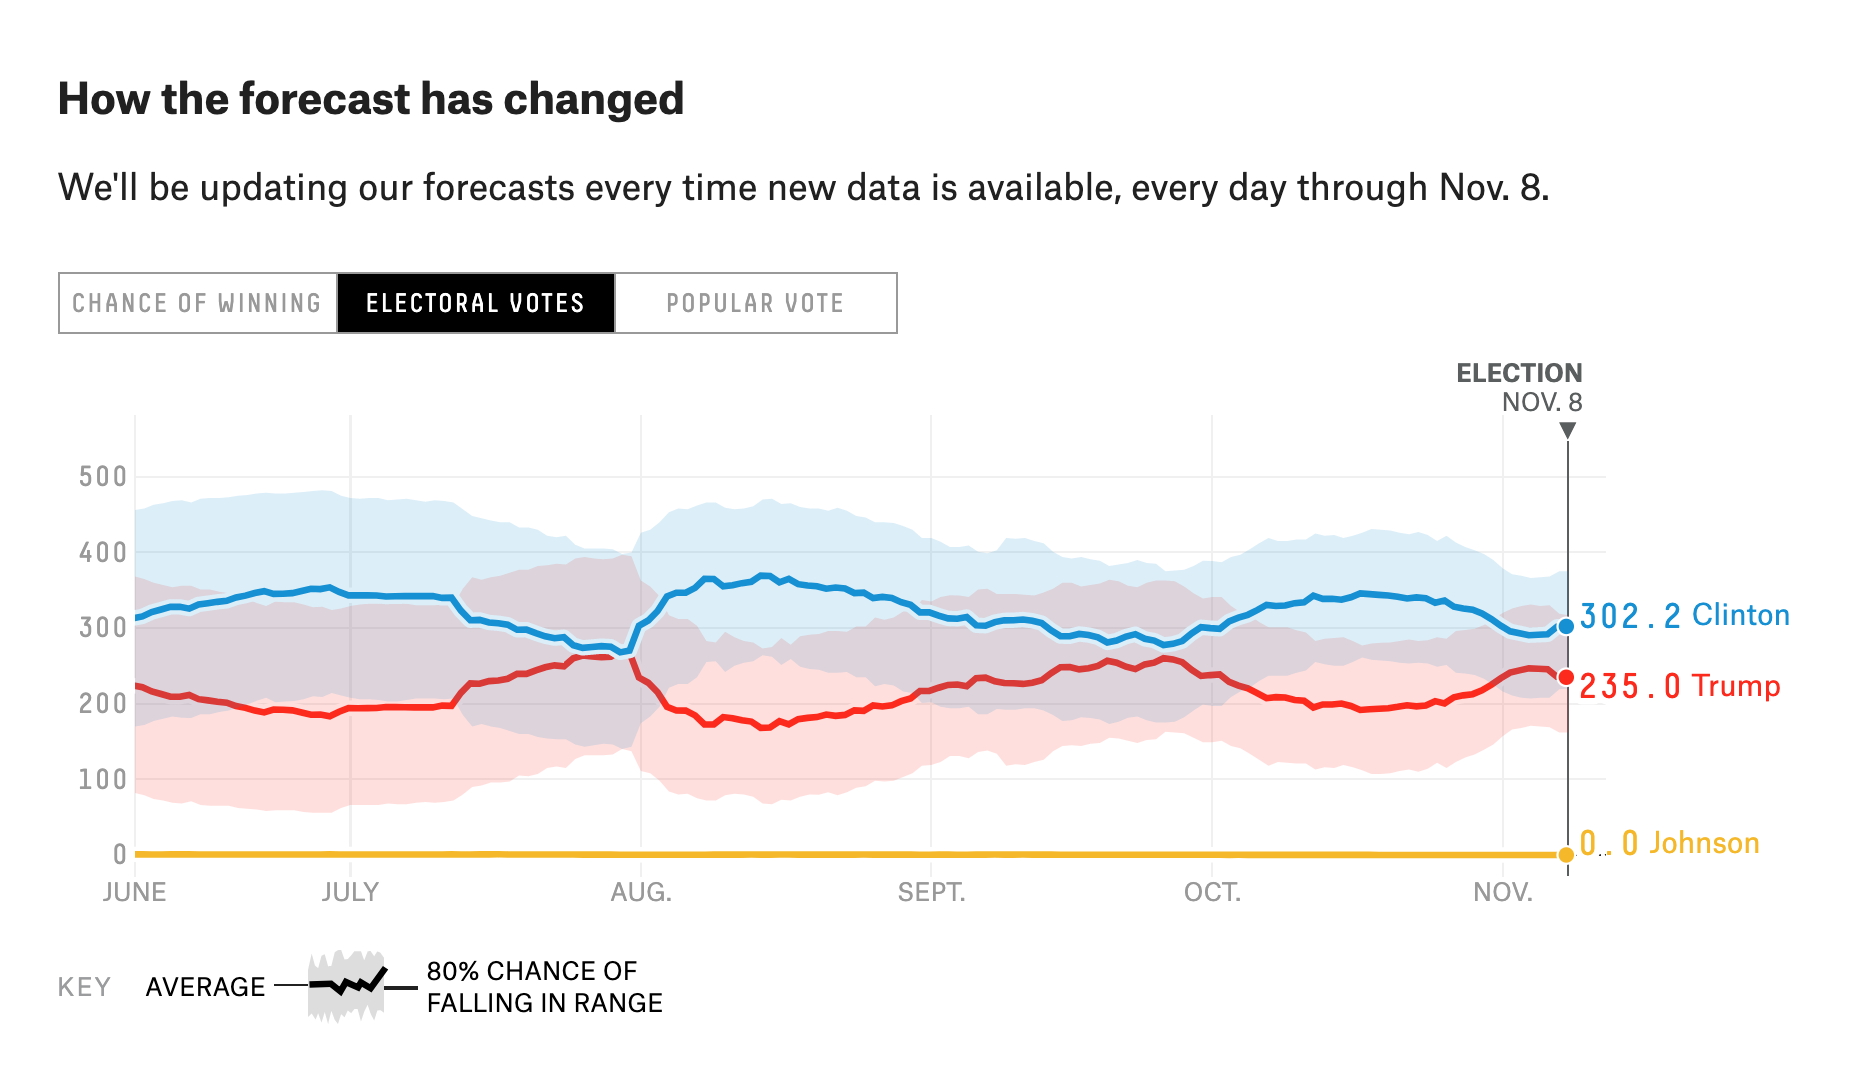
\includegraphics[scale=0.4]{forecast-ec.png}
\end{center}

\end{frame}

%@@@@@@@@@@@@@@@@@@@@@@@@@@@@@@@@@@@@@@@@@@@@@@@@@
\begin{frame}

\begin{center}
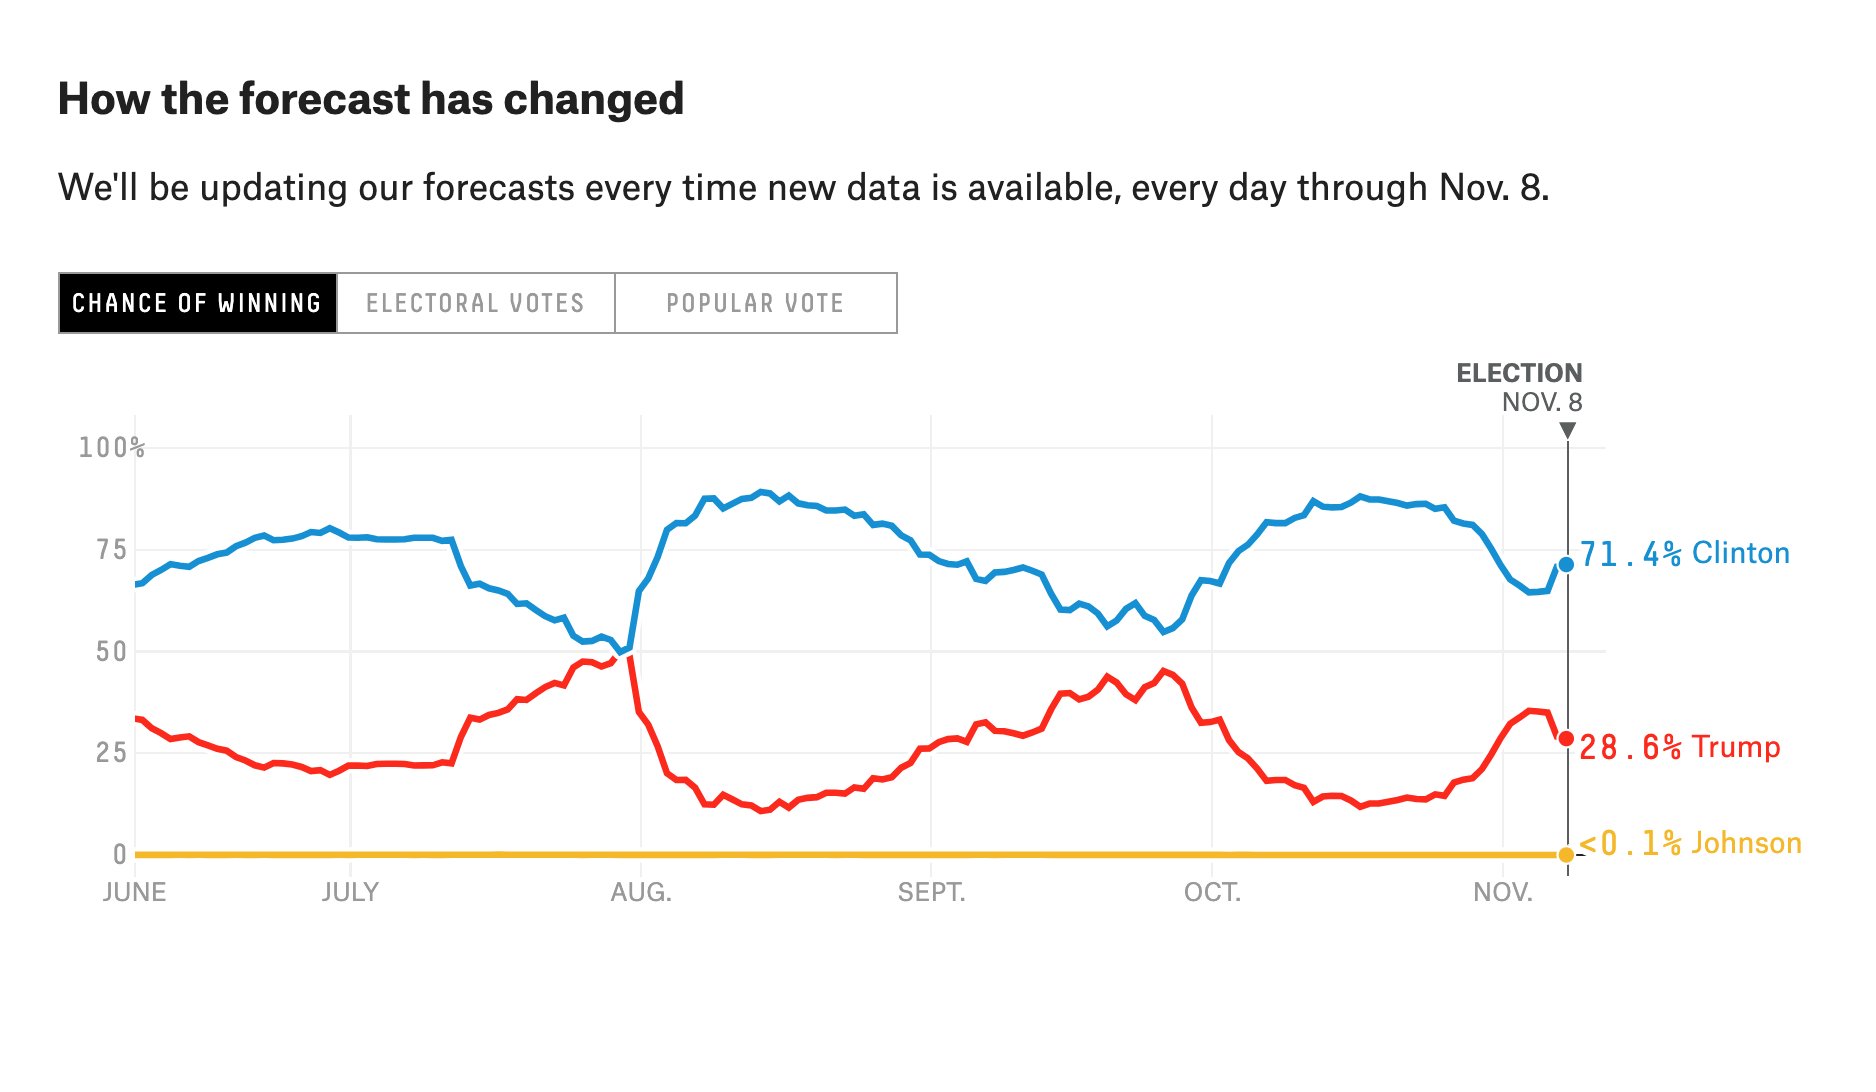
\includegraphics[scale=0.4]{forecast-win.png}
\end{center}

\end{frame}

%@@@@@@@@@@@@@@@@@@@@@@@@@@@@@@@@@@@@@@@@@@@@@@@@@
\begin{frame}
\frametitle{What does this $71/28$ probability mean?}

\begin{itemize}
\item Out of all the possible scenarios...
\begin{itemize}
\item In each state, either Trump or Clinton will win -- $2^{50}$ possibilities;
\item How many ways can you configure the electoral college map ($2^{50}$)?
\end{itemize}
\bigskip
\bigskip

\item ...that are consistent with our data...
\begin{itemize}
\item Not all scenarios are equally likely
\item We learn about the plausibility of scenarios from history and polls
\end{itemize}
\bigskip
\bigskip

\item ...how often is Clinton the winner?
\begin{itemize}
\item A poll has Clinton 1 pt. below Trump
\item What is the range over what Clinton's ``true vote" could be?
\item How many of the ``true votes" in that range are greater than Trump's?
\end{itemize}
\end{itemize}
\end{frame}

%%@@@@@@@@@@@@@@@@@@@@@@@@@@@@@@@@@@@@@@@@@@@@@@@@@
%\begin{frame}
%\frametitle{Blar}
%
%\begin{itemize}
%\item In regression, we use data to estimate \textbf{unknown population parameters}:
%\begin{align*}
%y = \beta_0 + \beta_1x1 + \beta_2x2 + \hdots + \varepsilon;
%\end{align*}
%\bigskip
%\bigskip
%
%\item In forecasting, we use polls to estimate \textbf{unknown population support};
%\begin{align*}
%  \text{State poll today} &= f\left( \text{True state vote today}, \text{Other} \right)
%\end{align*}
%\item Blar;
%\bigskip
%\bigskip
%
%\item Blar.
%
%\end{itemize}
%\end{frame}

%@@@@@@@@@@@@@@@@@@@@@@@@@@@@@@@@@@@@@@@@@@@@@@@@@
\begin{frame}
\frametitle{Building blocks}

\begin{columns}
\begin{column}{0.5\textwidth}

\begin{itemize}
\item FiveThirtyEight uses fundamentals (and historical data) to build ``prior expectations" for Election Day;
\begin{itemize}
\item Anchors each state as the model projects to Election Day;
\item Explores how each state differs from the average;
\item When state predictions are wrong, allows assessment of which states are ``wrong together;"
\end{itemize}
\bigskip

\item New polls ``update our prior expectations" about Election Day.
\end{itemize}

\end{column}
\begin{column}{0.5\textwidth}
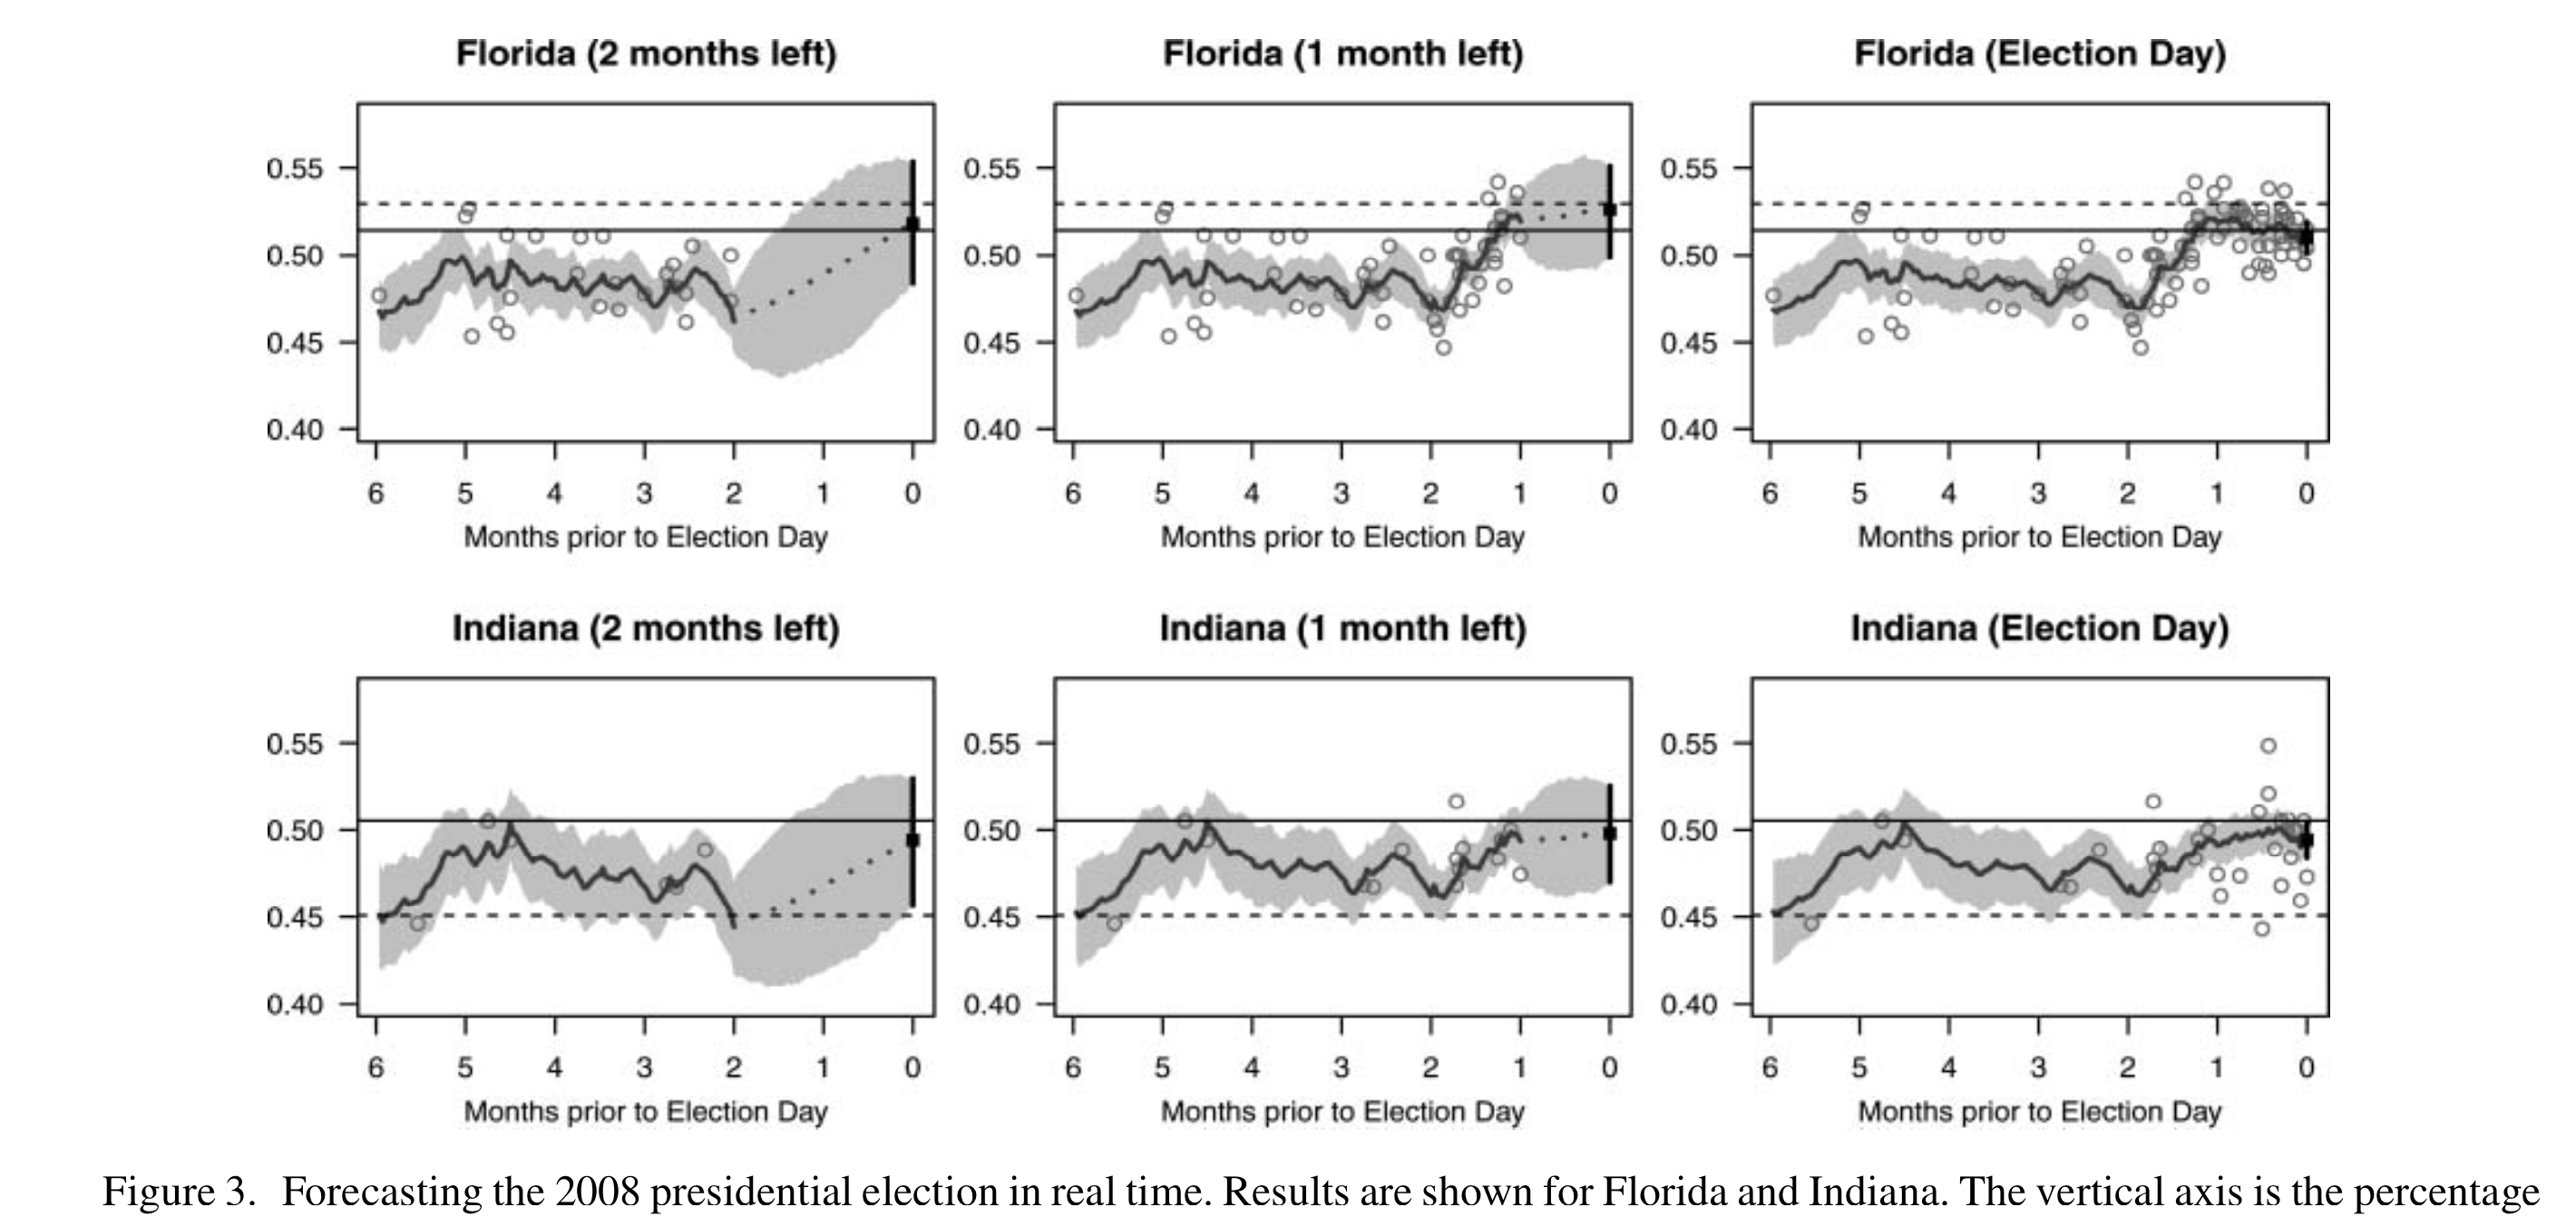
\includegraphics[scale=0.15]{random-walk.png}
\end{column}
\end{columns}

\end{frame}

%@@@@@@@@@@@@@@@@@@@@@@@@@@@@@@@@@@@@@@@@@@@@@@@@@
\begin{frame}
\frametitle{Awareness of uncertainty}
\begin{center}
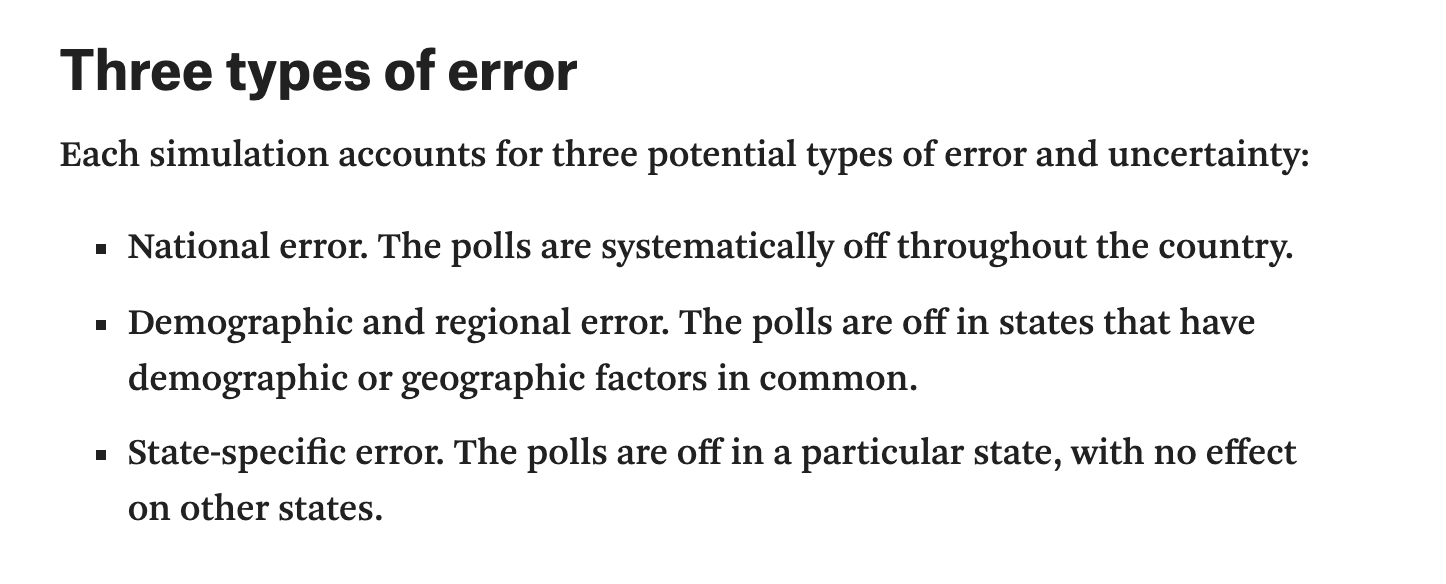
\includegraphics[scale=0.6]{538-errors.png}
\end{center}

\end{frame}

%@@@@@@@@@@@@@@@@@@@@@@@@@@@@@@@@@@@@@@@@@@@@@@@@@
\begin{frame}
\frametitle{What scenarios were compatible with the data?}
\begin{center}
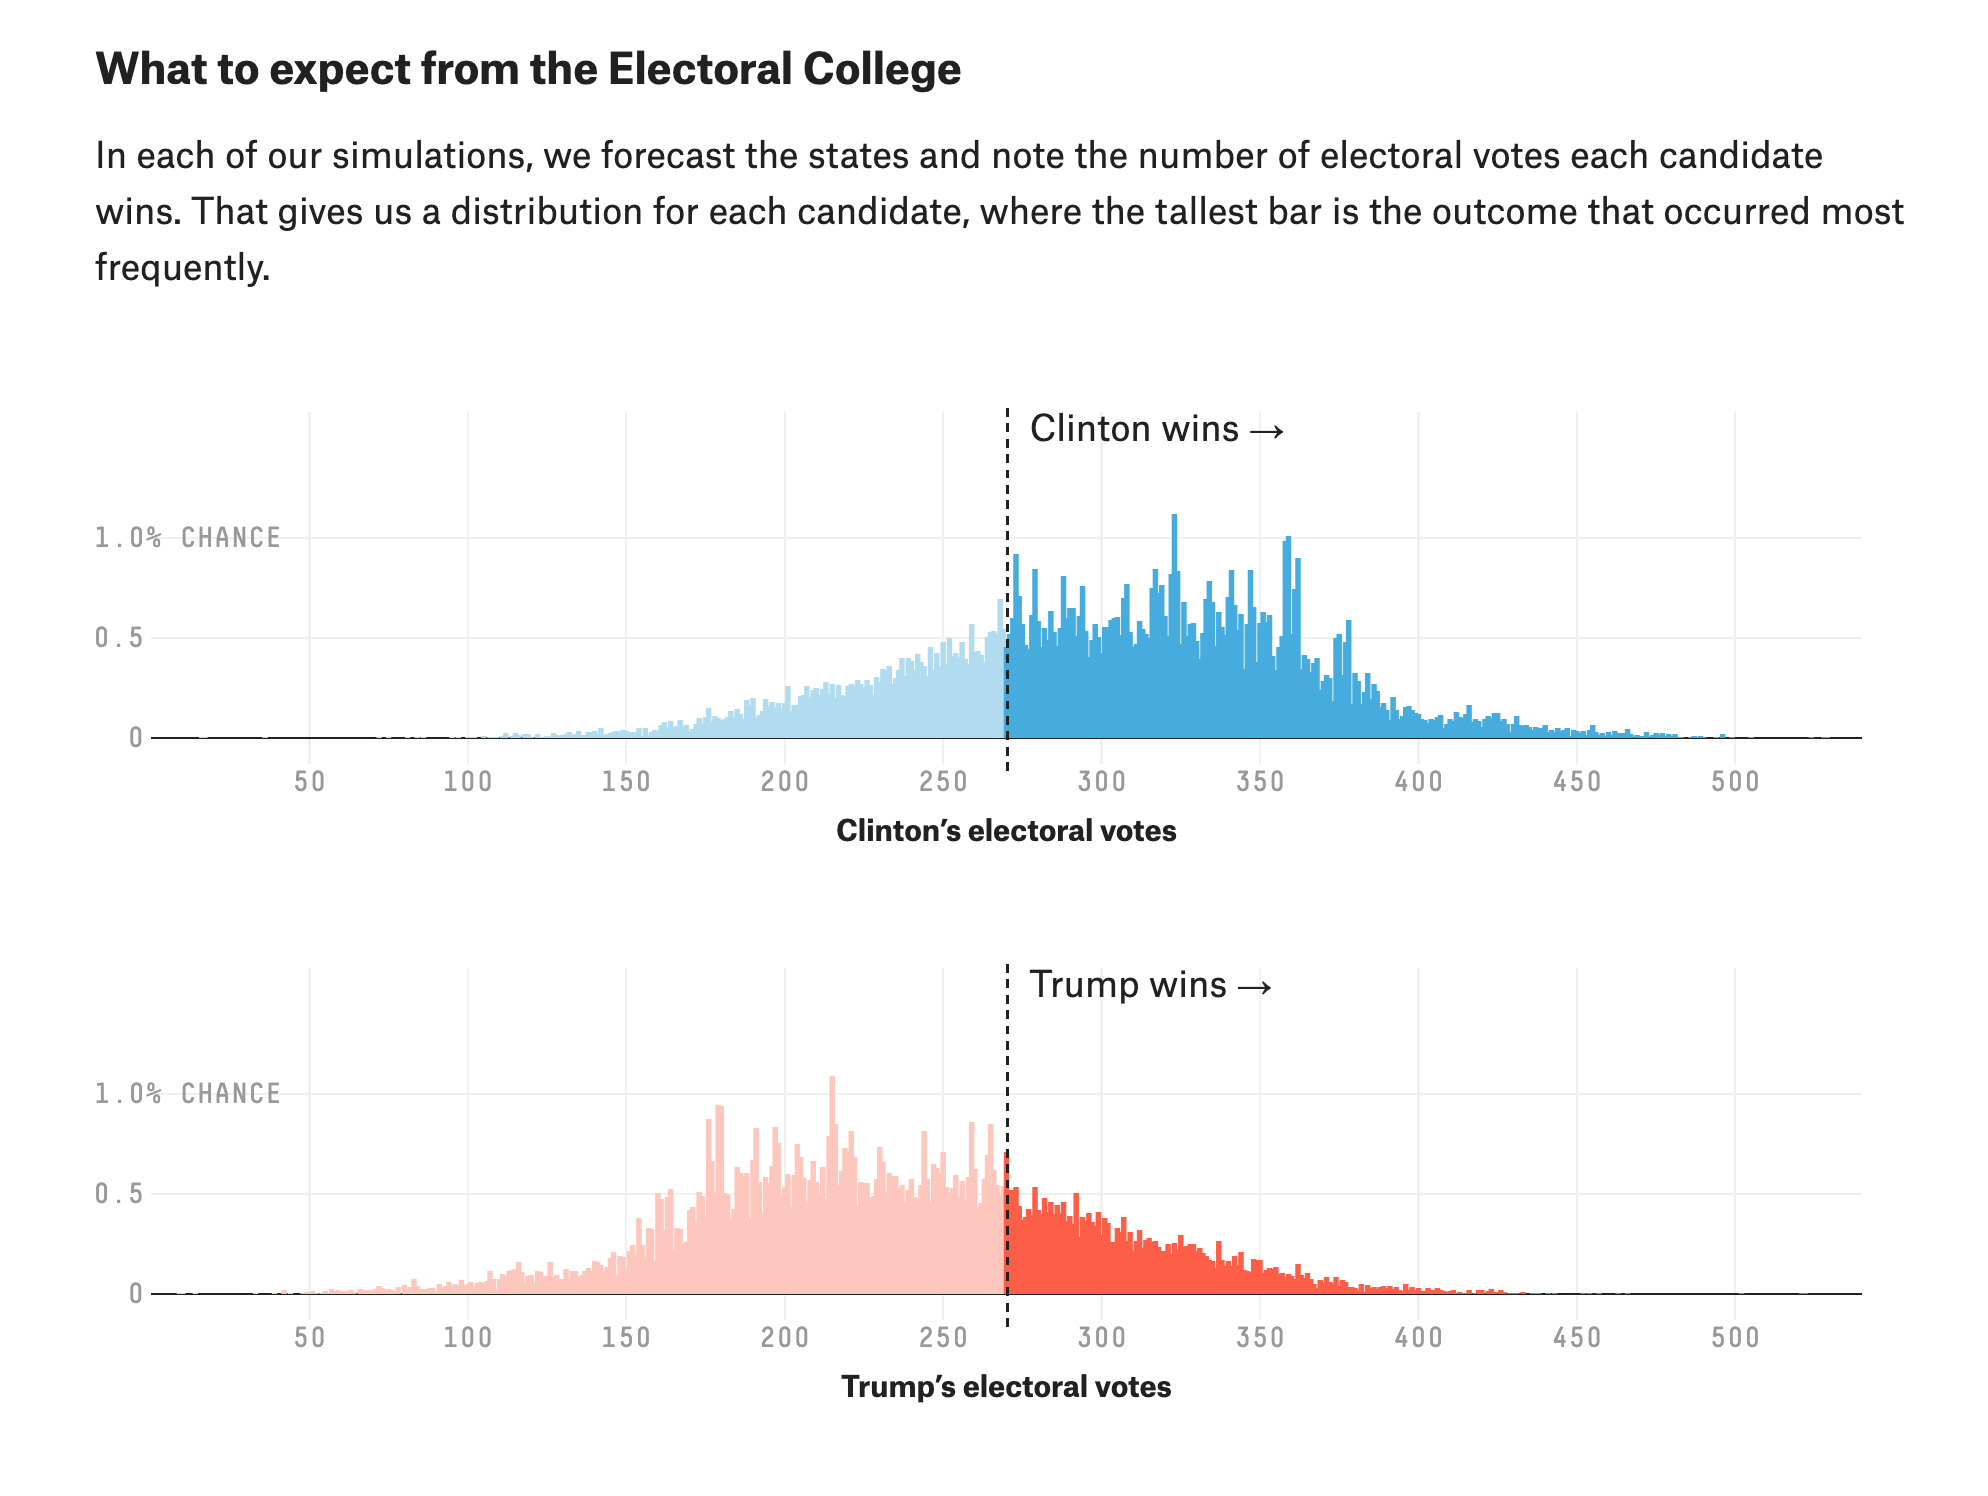
\includegraphics[scale=0.3]{ec-scenarios.png}
\end{center}

\end{frame}

%@@@@@@@@@@@@@@@@@@@@@@@@@@@@@@@@@@@@@@@@@@@@@@@@@
\begin{frame}
\frametitle{What scenarios were compatible with the data?}
\begin{center}
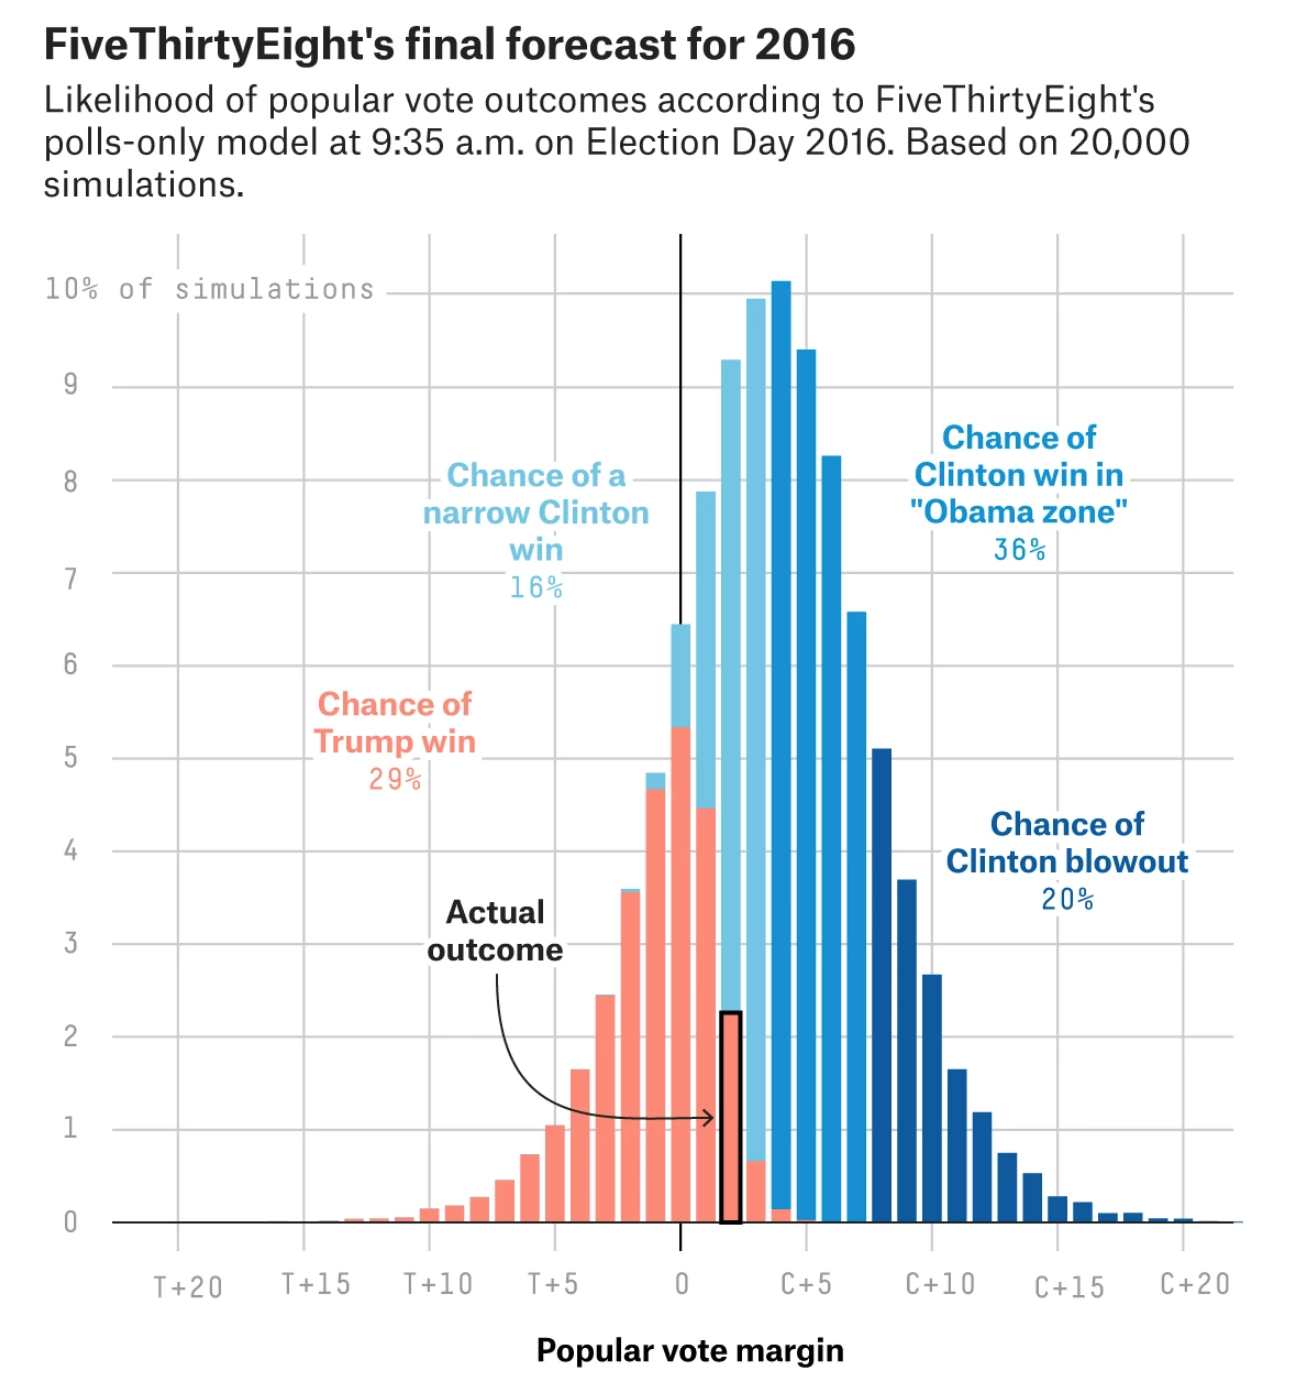
\includegraphics[scale=0.3]{as-f-popvote.png}
\end{center}

\end{frame}

%@@@@@@@@@@@@@@@@@@@@@@@@@@@@@@@@@@@@@@@@@@@@@@@@@
\begin{frame}
\frametitle{What scenarios were compatible with the data?}
\begin{center}
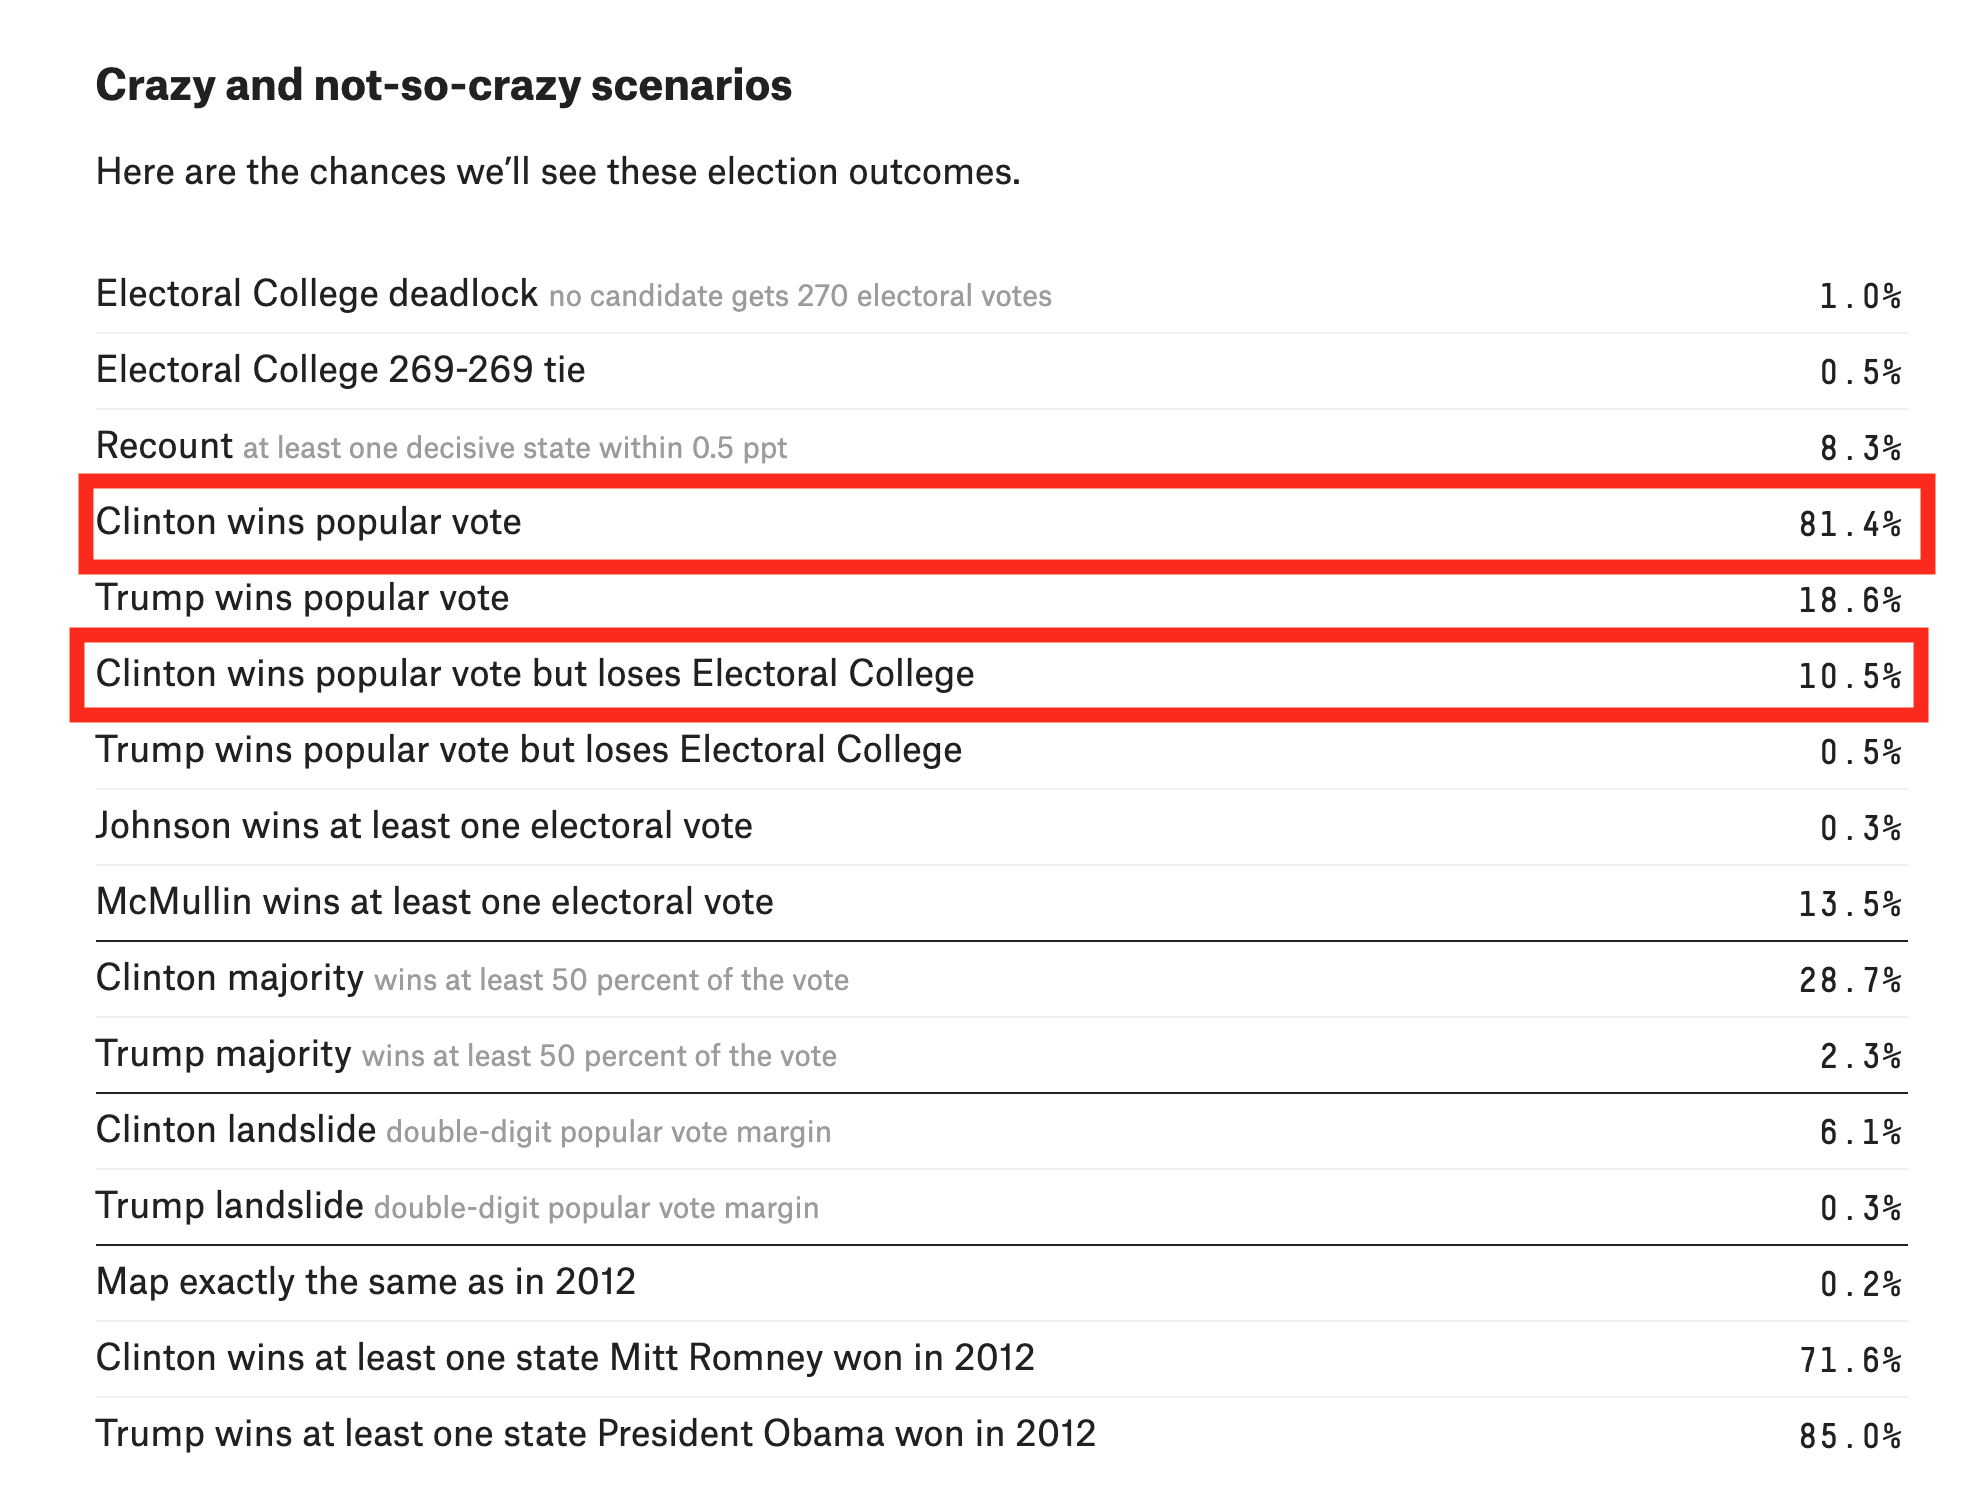
\includegraphics[scale=0.3]{scenarios.png}
\end{center}

\end{frame}

%@@@@@@@@@@@@@@@@@@@@@@@@@@@@@@@@@@@@@@@@@@@@@@@@@
\begin{frame}
\frametitle{What went wrong?!}

\begin{center}
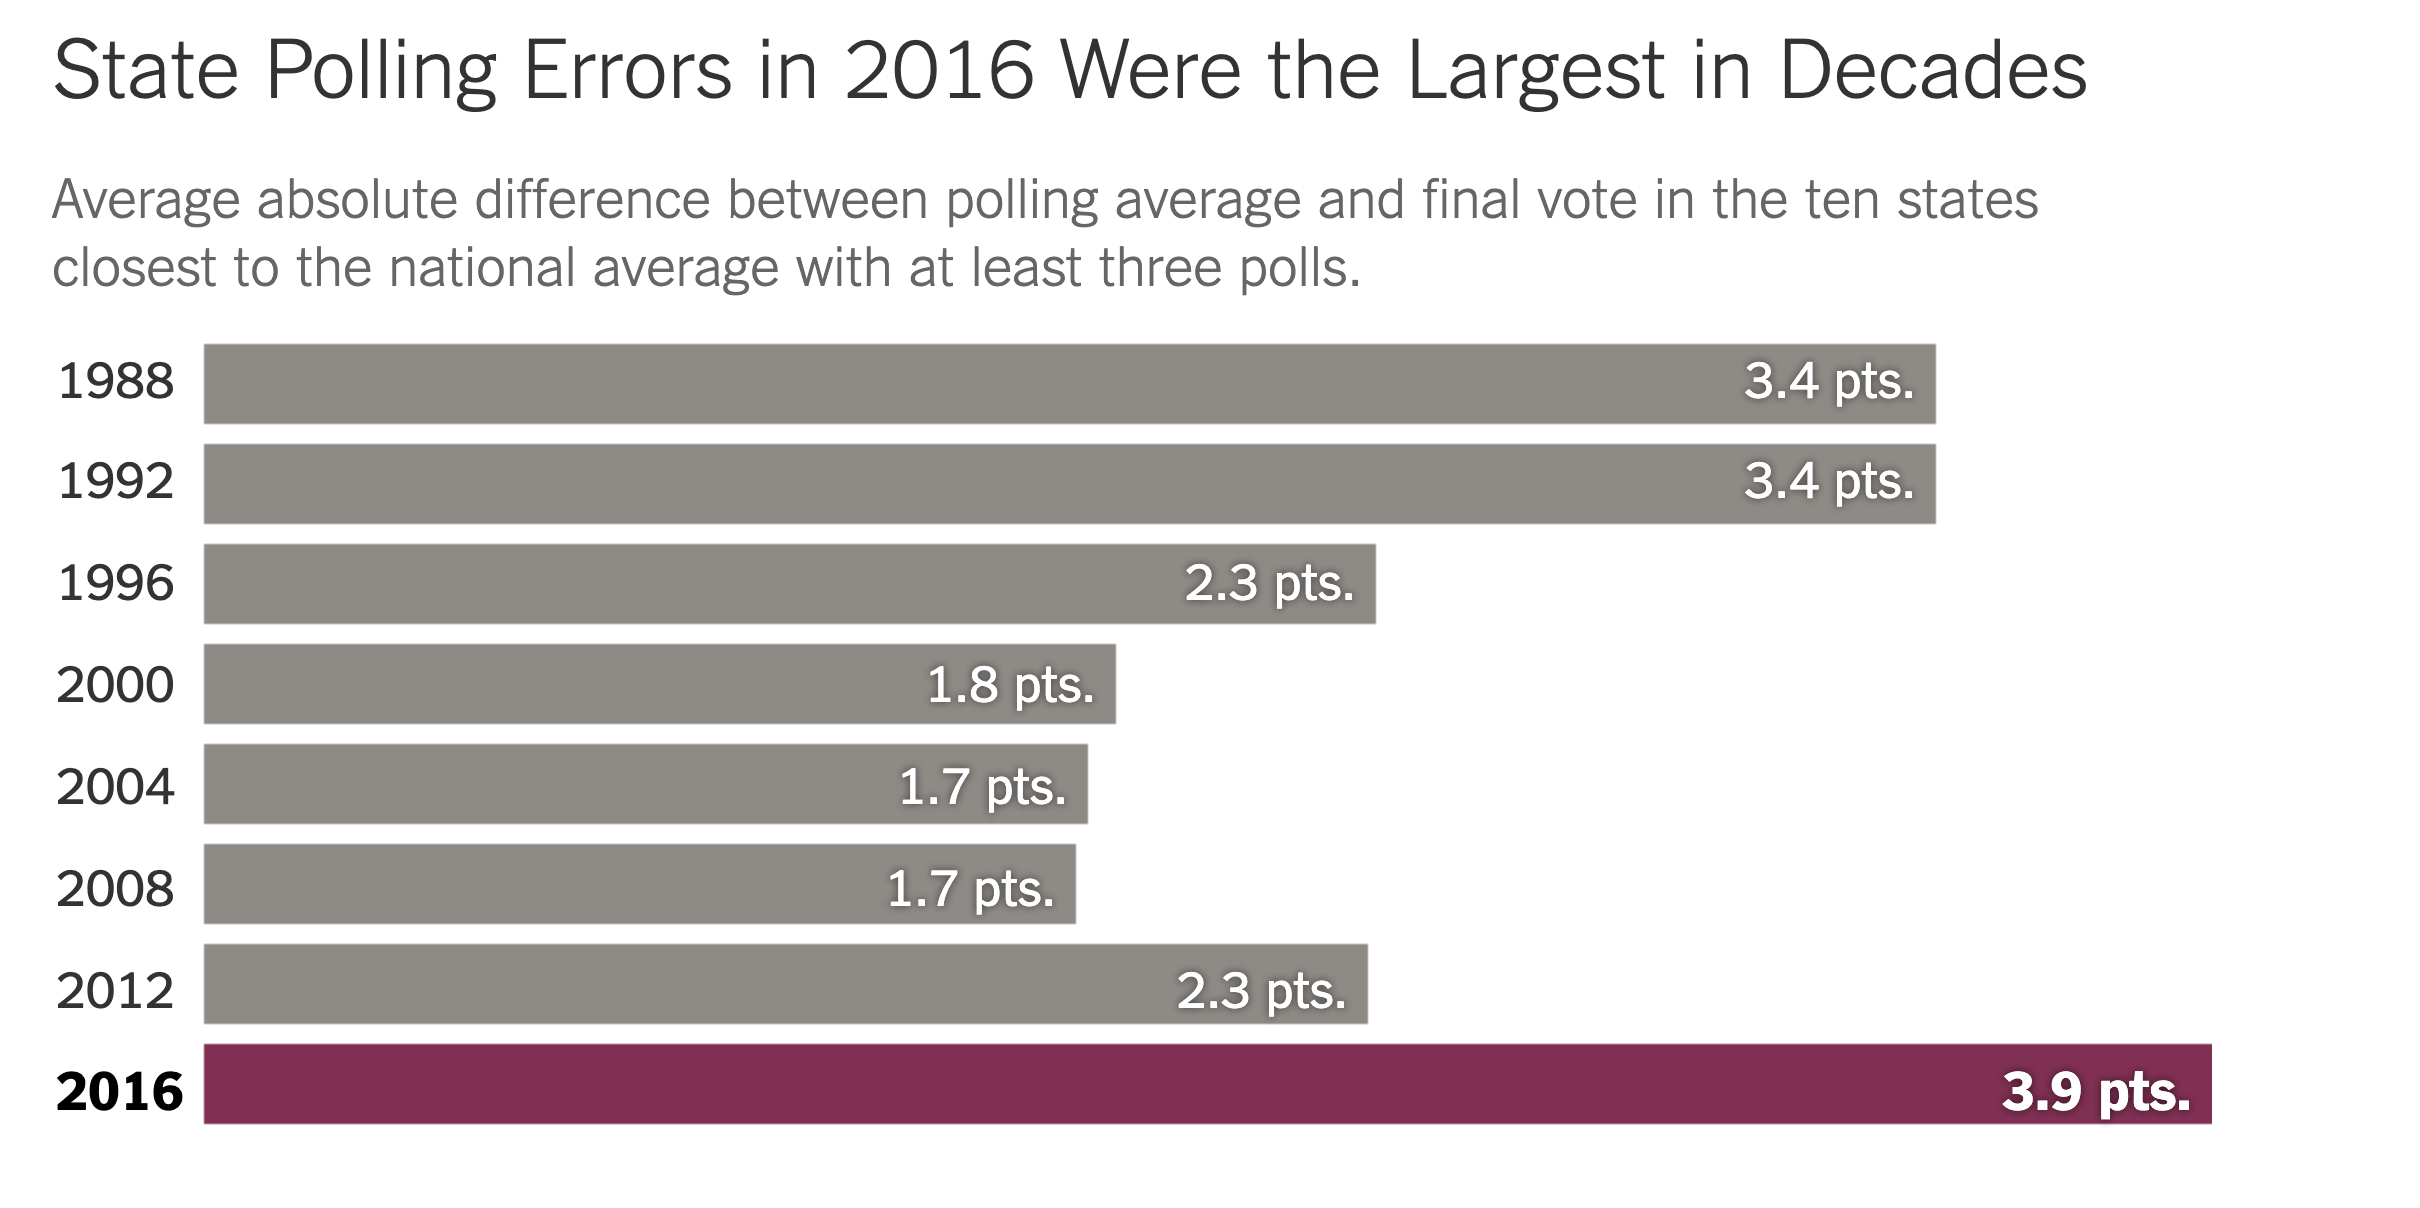
\includegraphics[scale=0.3]{state-errors.png}
\end{center}
\end{frame}

%@@@@@@@@@@@@@@@@@@@@@@@@@@@@@@@@@@@@@@@@@@@@@@@@@
\begin{frame}
\frametitle{Is forecasting good or bad?}

\begin{center}
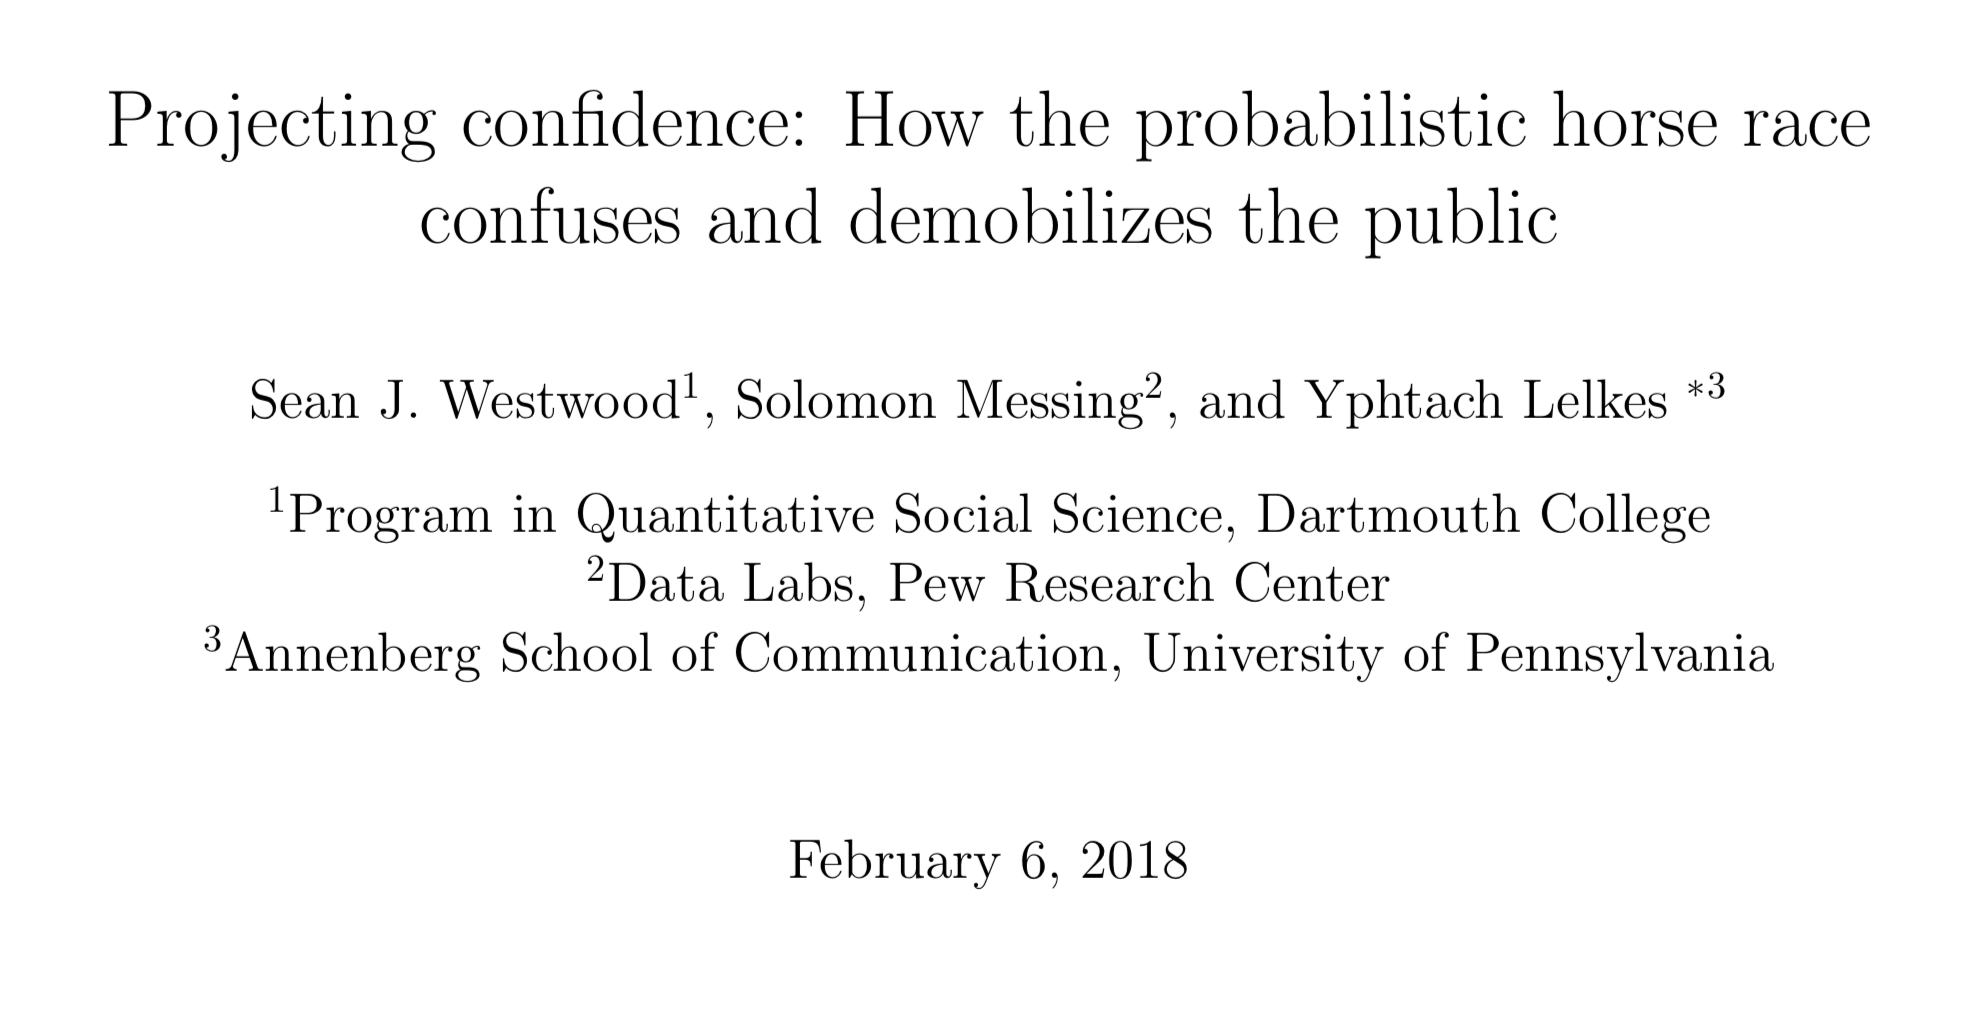
\includegraphics[scale=0.4]{uncertainty.png}
\end{center}
\end{frame}

%@@@@@@@@@@@@@@@@@@@@@@@@@@@@@@@@@@@@@@@@@@@@@@@@@
\begin{frame}

\begin{center}
\Huge\textbf{Assessment -- does your model predict well outside of the data on which it was made?}\\
\end{center}

\end{frame}

%%@@@@@@@@@@@@@@@@@@@@@@@@@@@@@@@@@@@@@@@@@@@@@@@@@
%\begin{frame}
%\frametitle{Linear Regresssion: Root Mean Squared Error}
%
%\begin{columns}
%\begin{column}{0.5\textwidth}
%
%\begin{itemize}
%\item We could measure model fit by looking at the `typical' error of the model when it makes predictions;
%\bigskip
%
%\item Remember how regression works?  It finds the $\beta$s by minimizing this:
%\begin{align*}
%\underbrace{\sum_i(\overbrace{y_i}^{\mbox{obs}} - \overbrace{(\beta_0 + \beta_1 x_i)}^{\mbox{prediction}})^2}_{\mbox{sum of squared residuals}}
%\end{align*}
%
%\item[] \color{white}\textbf{For HW7 root mean squared error: 3.390743.}
%\end{itemize}
%
%\end{column}
%\begin{column}{0.5\textwidth}
%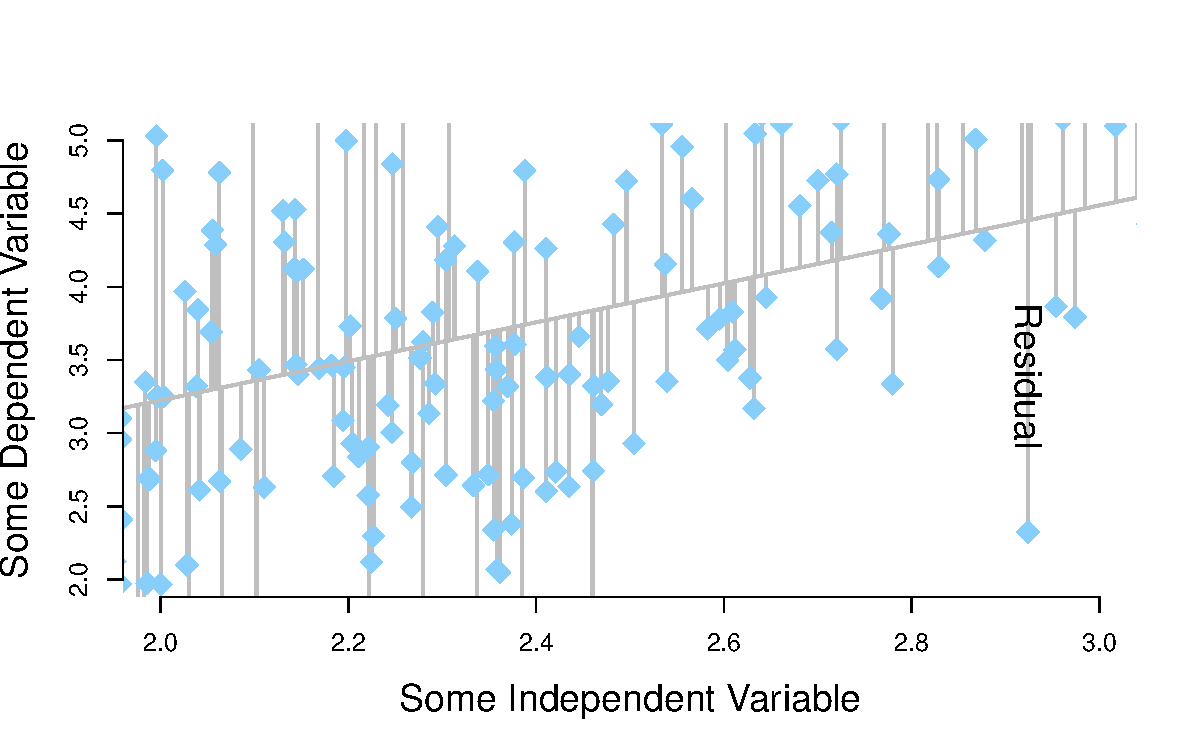
\includegraphics[scale=0.35]{point_cloud_line_zoomed_residuals.pdf}
%\end{column}
%\end{columns}
%
%\end{frame}

%@@@@@@@@@@@@@@@@@@@@@@@@@@@@@@@@@@@@@@@@@@@@@@@@@
\begin{frame}
\frametitle{How do we vet models?}

\begin{itemize}
\item Much of class has focused on \textbf{inference} -- our ability to reason about a \textbf{population} from a \textbf{sample};
\begin{itemize}
\item Average causal effect $=$ estimating general effects of a treatment;
\item Hypothesis testing $=$ inference about population parameters, e.g. the number of campaign supporters in the voting population;
\item Linear/logistic regression $=$ measuring the effect of an independent variable on a dependent variable;
\end{itemize}
\bigskip

\item[]\color{white} Something monumental happened last week -- as soon as we started to talk about `good' models we also started to talk about \textbf{prediction} rather than inference;
\begin{itemize}
\item[]\color{white} RMSE -- typical model \textbf{prediction} error;
\item[]\color{white} $R^2$ -- typical model \textbf{prediction} error compared with a naive model;
\item[]\color{white} $F$-test -- hypothesis test of fit (measured by \textbf{prediction} error);
\item[]\color{white} Confusion matrix -- binary \textbf{prediction} error aggregated across the data;
\item[]\color{white} Accuracy -- binary percent correctly \textbf{predicted};
\item[]\color{white} Precision/recall -- measurement of \textbf{prediction} quality;
\end{itemize}
\end{itemize}
\end{frame}

%@@@@@@@@@@@@@@@@@@@@@@@@@@@@@@@@@@@@@@@@@@@@@@@@@
\begin{frame}
\frametitle{How do we vet models?}

\begin{itemize}
\item Much of class has focused on \textbf{inference} -- our ability to reason about a \textbf{population} from a \textbf{sample};
\begin{itemize}
\item Average causal effect $=$ estimating general effects of a treatment;
\item Hypothesis testing $=$ inference about population parameters, e.g. the number of campaign supporters in the voting population;
\item Linear/logistic regression $=$ measuring the effect of an independent variable on a dependent variable;
\end{itemize}
\bigskip

\item Something monumental happened last week -- as soon as we started to talk about `good' models we also started to talk about \textbf{prediction} rather than inference;
\begin{itemize}
\item RMSE -- typical model \textbf{prediction} error;
\item $R^2$ -- typical model \textbf{prediction} error compared with a naive model;
\item $F$-test -- hypothesis test of fit (measured by \textbf{prediction} error);
\item Confusion matrix -- binary \textbf{prediction} error aggregated across the data;
\item Accuracy -- binary percent correctly \textbf{predicted};
\item Precision/recall -- measurement of \textbf{prediction} quality;
\end{itemize}
\end{itemize}
\end{frame}

%@@@@@@@@@@@@@@@@@@@@@@@@@@@@@@@@@@@@@@@@@@@@@@@@@
\begin{frame}
\frametitle{How do we vet models using out of sample work?}
\begin{enumerate}

\item Divide the data into a \textbf{training} set and a \textbf{test} set;
\begin{itemize}
\item No observations in common;
\item Test set is usually smaller;
\item Same dependent variable distribution across the two;
\end{itemize}
\bigskip
\bigskip

\item Create the model (e.g. linear regression) using the training data;
\bigskip
\bigskip

\item Use the model created with the training data to predict the test data -- compute metrics!

\end{enumerate}

\end{frame}

%@@@@@@@@@@@@@@@@@@@@@@@@@@@@@@@@@@@@@@@@@@@@@@@@@
\begin{frame}

\begin{center}
\Huge\textbf{Why should we care?}\\
\bigskip
\bigskip
\large Out of sample work is where the model becomes useful for helping us to control our world.\\
\end{center}

\end{frame}



\end{document}






